% CAMF: Continuity Anomaly Monitoring Framework
% MEng Computing Final Year Project Report
% Imperial College London - 2025
% Author: Mihail Buzadji
% CID: 01909514
% Supervisor: Dr Josiah Wang
% Second Marker: Dr Nuri Cingillioglu

\documentclass[11pt,a4paper,oneside]{book}

% Essential packages
\usepackage[utf8]{inputenc}
\usepackage[T1]{fontenc}
\usepackage{lmodern} % Modern Latin fonts
\usepackage[english]{babel}

% Page layout
\usepackage[top=2.5cm,bottom=2.5cm,left=3cm,right=2.5cm]{geometry}
\usepackage{setspace}
\onehalfspacing % Changed from double spacing for better readability

% Bibliography - using BibLaTeX with Vancouver style
\usepackage[
  backend=bibtex,
  style=vancouver,
  sorting=none,
  url=true,
  doi=false,
  eprint=false,
  maxbibnames=6,
  minbibnames=6,
  abbreviate=false,
  backref=false,
  defernumbers=true
]{biblatex}
\addbibresource{bibliography/references_vancouver.bib}

% Graphics and figures
\usepackage{graphicx}
\graphicspath{{figures/}}
\usepackage{subcaption}

% Tables
\usepackage{booktabs}
\usepackage{tabularx}

% Mathematics
\usepackage{amsmath}
\usepackage{amsfonts}
\usepackage{amssymb}

% Code listings
\usepackage{listings}
\lstdefinelanguage{JavaScript}{
  keywords={typeof, new, true, false, catch, function, return, null, catch, switch, var, if, in, while, do, else, case, break, const, let, async, await, class, extends, import, export, from},
  keywordstyle=\color{blue}\bfseries,
  ndkeywords={class, export, boolean, throw, implements, import, this},
  ndkeywordstyle=\color{darkgray}\bfseries,
  identifierstyle=\color{black},
  sensitive=false,
  comment=[l]{//},
  morecomment=[s]{/*}{*/},
  commentstyle=\color{purple}\ttfamily,
  stringstyle=\color{red}\ttfamily,
  morestring=[b]',
  morestring=[b]"
}
\lstset{
    basicstyle=\ttfamily\footnotesize,
    breaklines=true,
    captionpos=b,
    keepspaces=true,
    numbers=left,
    numbersep=5pt,
    showspaces=false,
    showstringspaces=false,
    showtabs=false,
    tabsize=2,
    frame=single,
    xleftmargin=15pt,
    framexleftmargin=15pt,
    framexrightmargin=0pt,
    framexbottommargin=4pt,
    backgroundcolor=\color{lightgray!10}
}

% Hyperlinks and cross-references
\usepackage[colorlinks=true,linkcolor=black,citecolor=black,urlcolor=blue]{hyperref}

% Headers and footers
\usepackage{fancyhdr}
\setlength{\headheight}{14pt} % Fix headheight warning

% Define page styles
\fancypagestyle{plain}{
  \fancyhf{}
  \fancyfoot[C]{\thepage}
  \renewcommand{\headrulewidth}{0pt}
  \renewcommand{\footrulewidth}{0pt}
}

\fancypagestyle{main}{
  \fancyhf{}
  \fancyhead[L]{\leftmark}
  \fancyhead[R]{\thepage}
  \renewcommand{\headrulewidth}{0.5pt}
  \renewcommand{\footrulewidth}{0pt}
}

% Page style for front matter chapters
\fancypagestyle{frontmatter}{
  \fancyhf{}
  \fancyhead[R]{\thepage}
  \renewcommand{\headrulewidth}{0pt}
  \renewcommand{\footrulewidth}{0pt}
}

% Chapter formatting - clean academic style
\usepackage{titlesec}
\titleformat{\chapter}[display]
  {\normalfont\huge\bfseries}
  {\chaptertitlename\ \thechapter}
  {20pt}
  {\Huge}
\titlespacing*{\chapter}{0pt}{0pt}{40pt}

% Format for unnumbered chapters in frontmatter
\newcommand{\frontmatterchapter}[1]{
  \cleardoublepage
  \phantomsection
  \addcontentsline{toc}{chapter}{#1}
  \chapter*{\hfill #1}
  \markboth{#1}{#1}
}

% Table of contents depth
\setcounter{tocdepth}{2}
\setcounter{secnumdepth}{3}

% Customize TOC appearance
\usepackage{tocloft}
\renewcommand{\cftchapfont}{\normalfont\bfseries}
\renewcommand{\cftchappagefont}{\normalfont\bfseries}
\renewcommand{\cftchapleader}{\cftdotfill{\cftdotsep}}
\renewcommand{\cftchapafterpnum}{\vskip5pt}
\setlength{\cftbeforechapskip}{10pt}

% Color package for any colored elements
\usepackage{xcolor}

% TikZ for positioning
\usepackage{tikz}

% Better enumeration
\usepackage{enumitem}

% Acronyms
\usepackage[withpage]{acronym}

% Appendix
\usepackage[toc,page]{appendix}

% Document metadata
\newcommand{\reporttitle}{CAM-F: Continuity Anomaly\texorpdfstring{\\}{ }Monitoring Framework}
\newcommand{\reportsubtitle}{Real-time Computer Vision-based System for Monitoring\\[0.3cm] On-set Film and Television Production}
\newcommand{\reportauthor}{Mihail Buzadji}
\newcommand{\reportcid}{01909514}
\newcommand{\reportdegree}{Master of Engineering}
\newcommand{\reportcourse}{Computing}
\newcommand{\reportsupervisor}{Dr Josiah Wang}
\newcommand{\reportsecondmarker}{Dr Nuri Cingillioglu}
\newcommand{\reportyear}{2025}
\newcommand{\reportdepartment}{Department of Computing}
\newcommand{\reportuniversity}{Imperial College London}

% PDF metadata
\hypersetup{
    pdftitle={\reporttitle},
    pdfauthor={\reportauthor},
    pdfsubject={MEng Computing Final Year Project},
    pdfkeywords={computer vision, film production, continuity monitoring, real-time systems}
}

\begin{document}

% Front matter
\frontmatter
\pagestyle{empty}

% Title page
\begin{titlepage}
    % Logo positioning (top left corner)
    \begin{tikzpicture}[remember picture, overlay]
        \node[anchor=north west, inner sep=0pt] at ([xshift=2.5cm, yshift=-2.5cm]current page.north west) {
            
\includegraphics[width=0.5\textwidth]{figures/IC_New_Logo.pdf}
        };
    \end{tikzpicture}
    
    \begin{center}
        \vspace*{3.5cm}
        
        % Institution - formal academic style
        {\Large \textbf{\reportuniversity}}\\[0.1cm]
        {\large \reportdepartment}
        
        \vspace{2.5cm}
        
        % Main title
        \doublespacing 
        {\huge \textsc{\reporttitle}} \par
        \singlespacing
        
        \vspace{0.8cm}
        
        % Subtitle
        {\Large \textsc{\reportsubtitle}}
        
        \vspace{4.0cm}
        
        % Author and Markers aligned with title width
        \begin{minipage}[t]{0.35\textwidth}
            \raggedright
            \textbf{Author}\\[2mm]
            {\large \textsc{\reportauthor}}\\[1mm]
            {\normalsize CID: \reportcid}
        \end{minipage}
        \hfill
        \begin{minipage}[t]{0.35\textwidth}
            \raggedleft
            \textbf{Supervised by}\\[2mm]
            {\large \textsc{\reportsupervisor}}\\[1mm]
            \vskip 1cm
            \textbf{Second Marker}\\[2mm]
            {\large \textsc{\reportsecondmarker}}
        \end{minipage}
        
        \vspace{1.5cm}
        
        % Date
        {\large June \reportyear}
        
        \vfill
        
        % Bottom text - formal submission statement
        \vspace{1cm}
        A Final Report submitted in fulfilment of requirements for the degree of\\[0.15cm]
        \textbf{\reportdegree\ in \reportcourse}
        
        \vspace{2.5cm}
    \end{center}
\end{titlepage}

% Set page style for front matter
\pagestyle{frontmatter}
\pagenumbering{roman}

% Abstract
% ABSTRACT WRITING GUIDELINES
% Based on analysis of distinguished MEng reports from Imperial College
%
% PURPOSE: The abstract is your report's elevator pitch. Someone reading ONLY the abstract
% must understand: (1) what problem you solved, (2) how you solved it, (3) what you achieved,
% and (4) why it matters. Maximum one page (~200-300 words).
%
% STRUCTURE (follow this exact order):
% 1. Context & Motivation (1-2 sentences): State the problem domain and why it matters
% 2. Gap/Challenge (1 sentence): What specific issue your project addresses
% 3. Approach & Methods (2-3 sentences): Your solution approach and key technical innovations
% 4. Key Results (2-3 sentences): Quantitative achievements and performance metrics
% 5. Implications (1-2 sentences): Significance and potential applications
%
% STYLE RULES:
% - NO CITATIONS in the abstract
% - Use present tense for facts ("Continuity errors cost...")
% - Use past tense for your work ("We developed...")
% - Be specific with numbers ("30fps processing", "95% accuracy", not "fast" or "accurate")
% - Define acronyms even if defined later ("CAMF (Continuity Anomaly Monitoring Framework)")
% - Avoid vague terms like "novel", "cutting-edge" without justification
%
% DISTINGUISHED PATTERNS TO EMULATE:
% - Start with a compelling industry/real-world problem
% - Clearly state what makes your approach unique (first to do X, combines Y and Z)
% - Include 2-3 specific technical contributions as bullets or integrated sentences
% - Provide concrete performance metrics from evaluation
% - End with broader impact beyond the immediate application
%
% COMMON MISTAKES TO AVOID:
% - Being too general or abstract
% - Focusing on implementation details rather than contributions
% - Missing quantitative results
% - Overselling ("revolutionary", "game-changing") without evidence
% - Writing an introduction instead of a summary
%
% EXAMPLE OPENING PATTERNS FROM DISTINGUISHED REPORTS:
% - "Film production continuity errors cost the industry £X million annually..."
% - "Current manual continuity supervision fails to detect Y% of errors..."
% - "The increasing complexity of modern productions requires..."

\frontmatterchapter{Abstract}

Continuity errors cost the film industry £620 million annually through reshoots and corrections, yet production teams rely on manual supervision methods that have been unchanged since the 1920s. Although existing research addresses only post-production analysis, no system provides real-time continuity monitoring during active filming, when errors can be prevented.

We present CAM-F (Continuity Anomaly Monitoring Framework), the first real-time continuity-monitoring system for film and television production. The framework uses a modular monolith architecture with process-isolated detector plugins, of which we developed two as proof-of-concept. ClockDetector combines the YOLOv11 object-detection model with ResNet50-based time prediction for analog clocks, and PaddleOCR for digital ones, whereas DifferenceDetector uses co-attention networks to identify prop changes.

Evaluation shows that ClockDetector processes a pair of frames in 1.92 seconds with 75.0\% accuracy, whereas DifferenceDetector achieves 60.7\% on change-detection benchmarks with 6.37 seconds of time to detection. The system enables real-time monitoring at 1.2 fps with both detectors enabled during the typical 5 minute reset periods between takes, proving that computer-assisted continuity supervision is viable during production.

CAM-F transforms continuity monitoring from expensive post-production correction to real-time prevention and establishes an extensible framework for specialised detector development. This addresses a critical gap in film-production pipeline, demonstrating how computer vision can augment, rather than replace, human expertise while potentially reducing industry costs.

% PLAIN LANGUAGE SUMMARY GUIDELINES
% Some departments require a plain language summary for accessibility
% Write for a general audience (your grandmother, a high school student)
% Avoid all technical jargon and explain the problem/solution simply
% Focus on real-world impact and relatable examples

\frontmatterchapter{Plain Language Summary}

Picture this: a paper coffee cup sitting on a medieval banquet table in your favourite fantasy drama, or Julia Roberts' breakfast croissant magically transforming into a pancake. These are called continuity errors and time-to-time they can break your immersion into the story, and beyond costing millions to fix, they can turn a high-budget production that took years to create into an internet meme overnight.

Film sets employ script supervisors to track every detail, but on complex productions with hundreds of people and constant changes, mistakes inevitably slip through. This project, CAM-F, acts as a digital assistant that helps catch these errors in real-time during filming.

Rather than building one massive system to catch every possible error, a framework was designed where specialised detectors can be added like plugins. One detector watches clocks to ensure time consistency, another spots when objects have moved between takes. The system alerts the script supervisor in real time, allowing fixes before moving on, rather than discovering problems months later when actors and sets are gone.

While computers can't replace the creative judgment of film professionals, this project shows how technology can make their jobs easier and help create better films with fewer costly mistakes.

% Acknowledgements
% Write your acknowledgements here
It is usual to thank those individuals who have provided particularly useful assistance, technical or otherwise, during your project.

This is not needed, but common.

% Table of contents
\cleardoublepage
\phantomsection
\addcontentsline{toc}{chapter}{Contents}
\renewcommand{\contentsname}{\hfill Contents}
\tableofcontents

% List of acronyms removed

% List of figures
\cleardoublepage
\phantomsection
\addcontentsline{toc}{chapter}{List of Figures}
\renewcommand{\listfigurename}{\hfill List of Figures}
\listoffigures

% List of tables (optional - uncomment if needed)
% \cleardoublepage
% \phantomsection
% \addcontentsline{toc}{chapter}{List of Tables}
% \renewcommand{\listtablename}{\hfill List of Tables}
% \listoftables

% Main matter
\mainmatter
\pagestyle{main}
\pagenumbering{arabic}

% Chapters
\chapter{Introduction}
\label{ch:introduction}

Film production represents a complex orchestration of creative and technical elements where minor inconsistencies can undermine narrative coherence. Among production challenges, continuity errors occupy a unique position: easily preventable during principal photography yet expensive to correct in post-production. This project investigates whether computer-vision technologies can assist human supervisors in detecting these anomalies in real-time on-set.

\section{The Continuity Problem in Film Production}
\label{sec:continuity_problem}

Maintaining continuity in film production proves surprisingly complex. A single scene often requires multiple takes, set reconstructions and extended breaks between shooting sessions. Each interruption increases risk of unintentional inconsistencies: a mug shifting position on a table, an actor's shirt changing from checkered to striped pattern, or a clock showing impossible time progression. These errors, known collectively as continuity errors, undermine narrative coherence and damage production credibility.

The global film- and video-production industry, valued at approximately £200 billion annually~\cite{businessresearch2025}, faces persistent quality-control challenges. Among these, continuity errors are a particularly costly problem. These visual inconsistencies between shots, ranging from misplaced props to temporal impossibilities, require expensive post-production corrections when discovered late in the pipeline. Industry professionals estimate that major productions allocate 5–10\% of post-production budgets specifically to continuity-related fixes~\cite{filmustage2024}, although comprehensive industry-wide cost data remains unavailable.

With more than 9,000 theatrical films produced globally each year~\cite{wipo2025}, plus countless television episodes and streaming content, the cumulative impact of continuity errors affects thousands of productions. Despite mature computer-vision capabilities in adjacent domains, no automated system currently assists the thousands of script supervisors worldwide who manually track continuity during filming on their own.

\section{The Technical Challenge}
\label{sec:technical_challenge}

Recent advances in computer vision suggest potential for automated assistance. Object detection algorithms achieve high accuracy and performance on standard benchmarks~\cite{tsirtsakis2025}. However, continuity detection during film production presents unique challenges that differentiate it from conventional video analysis:

\textbf{Temporal discontinuity}: Unlike surveillance or sports analysis, in which frames flow continuously, film production captures scenes out of sequence. Shots requiring continuity matching might be filmed days or weeks apart, invalidating assumptions about temporal coherence that underpin most video-processing algorithms.

\textbf{Semantic ambiguity}: Determining whether a visual change constitutes an error requires understanding narrative context. A change in a character's appearance might represent deliberate storytelling or a continuity mistake. Current technologies lack the contextual reasoning to make these distinctions reliably.

\textbf{Real-time constraints}: Film sets operate on tight schedules in which every minute costs hundreds of pounds. Any detection system must operate inside the natural rhythm of production, without adding any overhead.

\textbf{Security requirements}: Film footage represents valuable intellectual property. Productions implementing automated systems require guarantees against data exfiltration, particularly when using community-contributed detection algorithms.

\section{Research Gap}
\label{sec:research_gap}

A literature review reveals minimal prior work addressing real-time continuity detection. Pickup and Zisserman's 2009 study~\cite{pickup2009} represents the sole academic attempt, analysing completed films to rank potential continuity errors. Their SIFT-based approach, although groundbreaking for its time, had several limitations in practicality.

The absence of subsequent research might stem from three factors. First, the film industry's closed nature limits academic access to production footage and workflows. No public datasets exist for training or evaluation, because productions rarely release raw footage. Second, the interdisciplinary nature of the problem, requiring both computer-vision expertise and film-production knowledge, creates barriers. Third, niche application of the advanced research computer-vision technologies in film is not as appealing as other more impactful industries.

To fill the gap this project addresses 2 main questions:
\begin{enumerate}
\item Can we build a system that can monitor footage on-set in real time?
\item Would it accurately detect common continuity anomalies within the production constraints?
\end{enumerate}

\section{Contributions}
\label{sec:contributions}

This project makes three primary contributions:

\begin{enumerate}
\item \textbf{Near production-ready deployment system}: We developed a complete, deployable application that integrates seamlessly with existing film-production workflows. The system installs in under a few minutes on a standard laptop, requires a connection to the camera or any source that streams the footage from it and no technical expertise. Unlike research prototypes, CAM-F is immediately usable on film sets without disrupting established production pipeline.

\item \textbf{Secure detector plugin framework}: We develop a modular detector framework using Docker containerisation with comprehensive security measures. This enables safe execution of community-contributed detectors without risking footage exfiltration.

\item \textbf{Validated detector implementations}: We implement two detectors addressing different error types. ClockDetector identifies temporal inconsistencies in clocks with 74.95\% accuracy and 1.92 seconds to detection, and DifferenceDetector locates spatial changes at 60.7\% accuracy with 6.37 seconds to detection. These establish baseline performance metrics for future research.
\end{enumerate}

Along with the main contributions, due to the novel nature of this specialised application field, we have contributed a simple tailored metric for evaluation of the detectors' practical performance in real-world deployment scenarios.

% Note: Thesis structure section removed as per the main content provided
\chapter{Background}
\label{ch:background}

\section{Understanding Continuity Anomalies}

\subsection{Definitions and guidelines}

Before proceeding with the discussion of continuity in film, let's establish the following:

Frame is a single static image captured by the camera. Displayed sequentially at a usual standard rate of 24 frames per second, it creates the perception of continuous motion.

Take is a single video recording from the moment the camera starts rolling until it stops. Typically multiple takes of the same action are filmed to capture the best possible shots and to provide coverage from different camera angles required for the scene.

Shot is a continuous sequence of frames, retrieved from the take. It serves as a distinct segment between cuts in the final edit, forming a scene.

Scene consists of multiple shots usually set in the same location and time, representing a distinct narrative moment within the film.

Continuity encompasses a wide range of visual and narrative details that should remain consistent across a scene. There are established guidelines in the industry that help maintain it~\cite{miller1999}. For example, a well-known continuity rule is where clocks, watches, or phone displays in a scene must show the same time across different shots if they represent the same narrative moment. Another common rule is to match eyelines between shots to ensure that the character's gaze aligns correctly with whatever or whoever they are looking at. In the video for VanityFair~\cite{vanityfair2023} Martin Scorsese's long-time script supervisor Martha Pinson showcased a few of the main things she looks out for in a film (see Figure 2.1).

\begin{figure}[h]
\centering
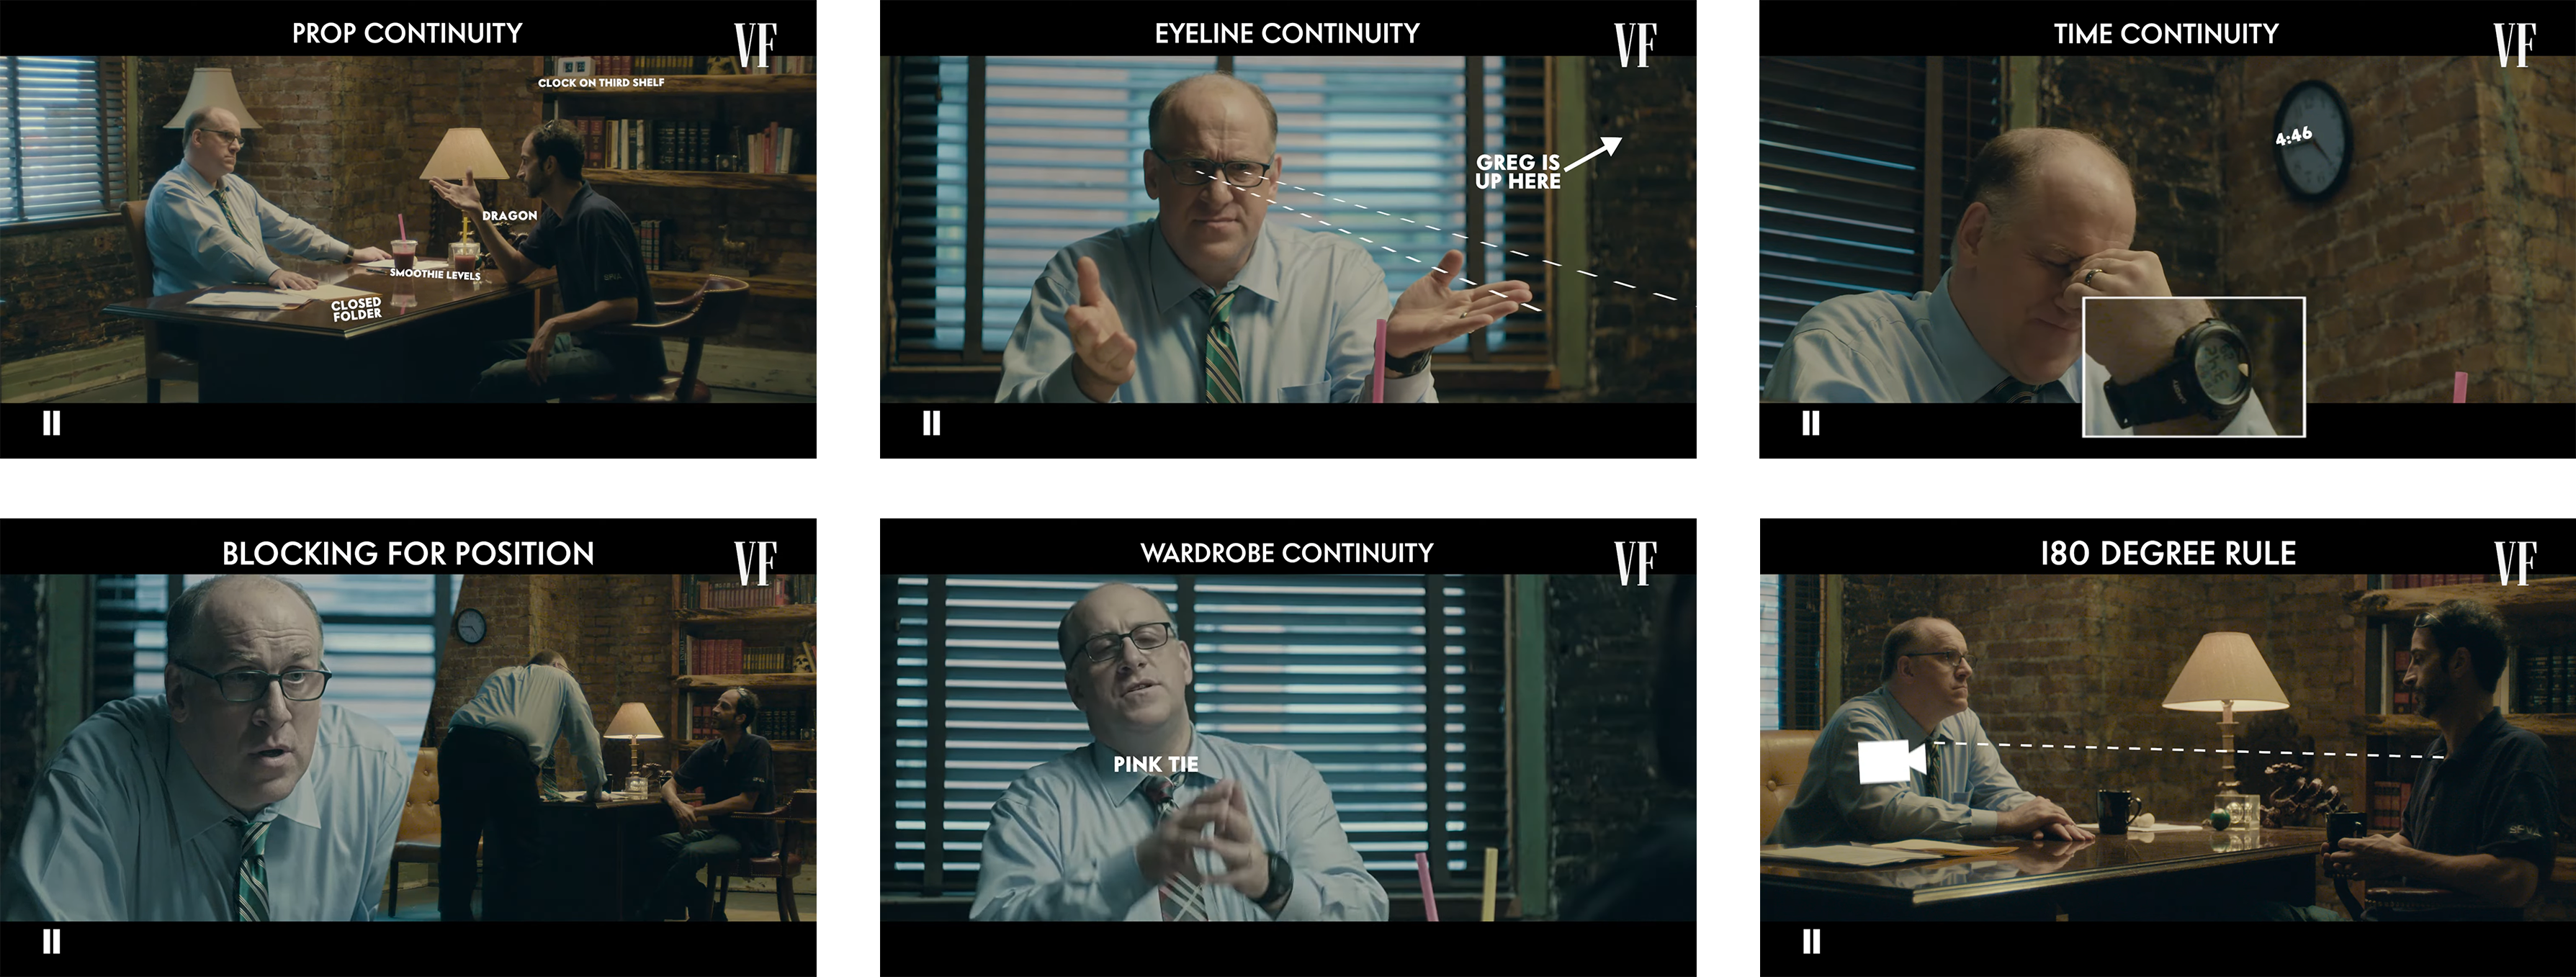
\includegraphics[width=0.8\textwidth]{figures/VF-Continuity.png}
\caption{Examples of continuity rules monitored by script supervisors. Top row (left to right): prop continuity, eyeline continuity, time continuity. Bottom row (left to right): blocking for position, wardrobe continuity, 180-degree rule. Source:~\cite{vanityfair2023}}
\label{fig:continuity-examples}
\end{figure}

\subsection{Variation in continuity errors}

Pat P. Miller in his book "Script Supervising and Film Continuity" defines it as "the art and craft of maintaining consistency in every visual and aural detail from shot to shot"~\cite{warm2008}. This definition encompasses multiple error categories requiring different detection approaches. Table 2.1 categorises these error types with their characteristics and typical manifestations.

\begin{table}[h]
\centering
\begin{tabularx}{\textwidth}{|l|X|X|}
\hline
\textbf{Error Type} & \textbf{Description} & \textbf{Common Examples} \\
\hline
Temporal Continuity & Inconsistent time progression within scenes that should represent continuous action & 
\begin{itemize}[nosep,leftmargin=*]
\item Clock faces showing impossible time jumps
\item Candle lengths increasing between shots
\item Daylight changes within supposedly continuous action
\item Weather variations during single conversations
\end{itemize} \\
\hline
Spatial Continuity & Incorrect object placement and positioning between shots & 
\begin{itemize}[nosep,leftmargin=*]
\item Props appearing or disappearing between shots
\item Costume elements changing state (buttons, zippers, accessories)
\item Character positions jumping unnaturally
\item Background elements shifting location
\end{itemize} \\
\hline
Action Continuity & Broken physical movement flow across edits & 
\begin{itemize}[nosep,leftmargin=*]
\item Gestures not matching across cuts
\item Objects held in different hands
\item Incomplete actions (drinking, smoking, eating)
\item Mismatched movement directions
\end{itemize} \\
\hline
Technical Continuity & Unintended production elements visible in final footage & 
\begin{itemize}[nosep,leftmargin=*]
\item Crew reflections in surfaces
\item Equipment visible in frame
\item Lighting inconsistencies
\item Focus or exposure jumps
\end{itemize} \\
\hline
\end{tabularx}
\caption{Classification of continuity errors in film production with descriptions and common examples}
\label{tab:continuity-errors}
\end{table}

\section{The Cognitive Science of Continuity Supervision}

\subsection{Vigilance Task Characteristics}

Script supervision exemplifies a sustained vigilance task, a category extensively studied in cognitive psychology. Warm, Parasuraman and Matthews demonstrated that vigilance tasks impose significant cognitive load, with performance typically declining 10–30\% within the first 30–60 minutes of sustained attention~\cite{see1997}. This 'vigilance decrement' occurs across diverse monitoring tasks, from radar operation to quality-control inspection. Film production amplifies these challenges through several factors:

Extended duration: Production days typically span 10–14 hours, far exceeding experiment designs of laboratory vigilance studies. Script supervisors must maintain attention across this entire period, often with minimal breaks between setups.

Information overload: Modern 4K cameras capture 8.3 million pixels per frame at 24–30 frames per second. In this data stream, supervisors track dialogue delivery, actor positions, prop placement, wardrobe details and temporal elements simultaneously. This can be overwhelming to track for one supervisor.

Low signal prevalence: Actual continuity errors occur relatively rarely. Signal-detection theory predicts that low target prevalence shifts response criteria, increasing miss rates. When errors are uncommon, maintaining sensitivity becomes cognitively demanding.

Working memory taxation: Non-linear shooting schedules require supervisors to maintain mental models of narrative chronology while observing out-of-sequence filming. This dual-task paradigm markedly affects detection performance.

Script supervisors use various mitigation strategies including photographic documentation, detailed notes and systematic checking procedures to reduce error rates~\cite{grier2003}.

\section{Film Production Workflows}

\subsection{Production Constraints}

Understanding production workflows proves essential for system design. Film sets operate on carefully orchestrated schedules where delays cascade expensively. Whereas simple changes to a set can take just a few minutes, larger-scale lighting or camera adjustments can take up to half an hour; on average, a regular reset between takes is about 5 minutes. These windows define the timeline in which continuity anomalies are usually corrected and another set of notes is recorded. A system requiring too long to process the footage on a small production with short reset periods would miss the prevention opportunities, rendering it impractical.

\subsection{Tools and Practices}

Script supervisors currently employ a hybrid analogue–digital workflow that combines modern technology with traditional methods (see Figure 2.2). Digital systems, particularly ScriptE~\cite{scriptesystems2024}, have become the dominant tool in professional productions, providing iPad-based interfaces that enable supervisors to log takes, track coverage and annotate scripts efficiently. However, these systems lack automated error-detection capabilities, requiring supervisors to rely entirely on manual observation.

Additionally, supervisors use digital cameras extensively to capture reference images for each setup, creating comprehensive visual documentation of props, wardrobe, makeup, actor positions and set arrangements~\cite{scriptation2025}. This multi-tool approach extends to team coordination, where supervisors must communicate with multiple departments including costume, props and makeup. Each department maintains its own continuity records, which creates beneficial redundancy but also introduces the potential for inconsistencies across documentation systems.

\begin{figure}[h]
\centering
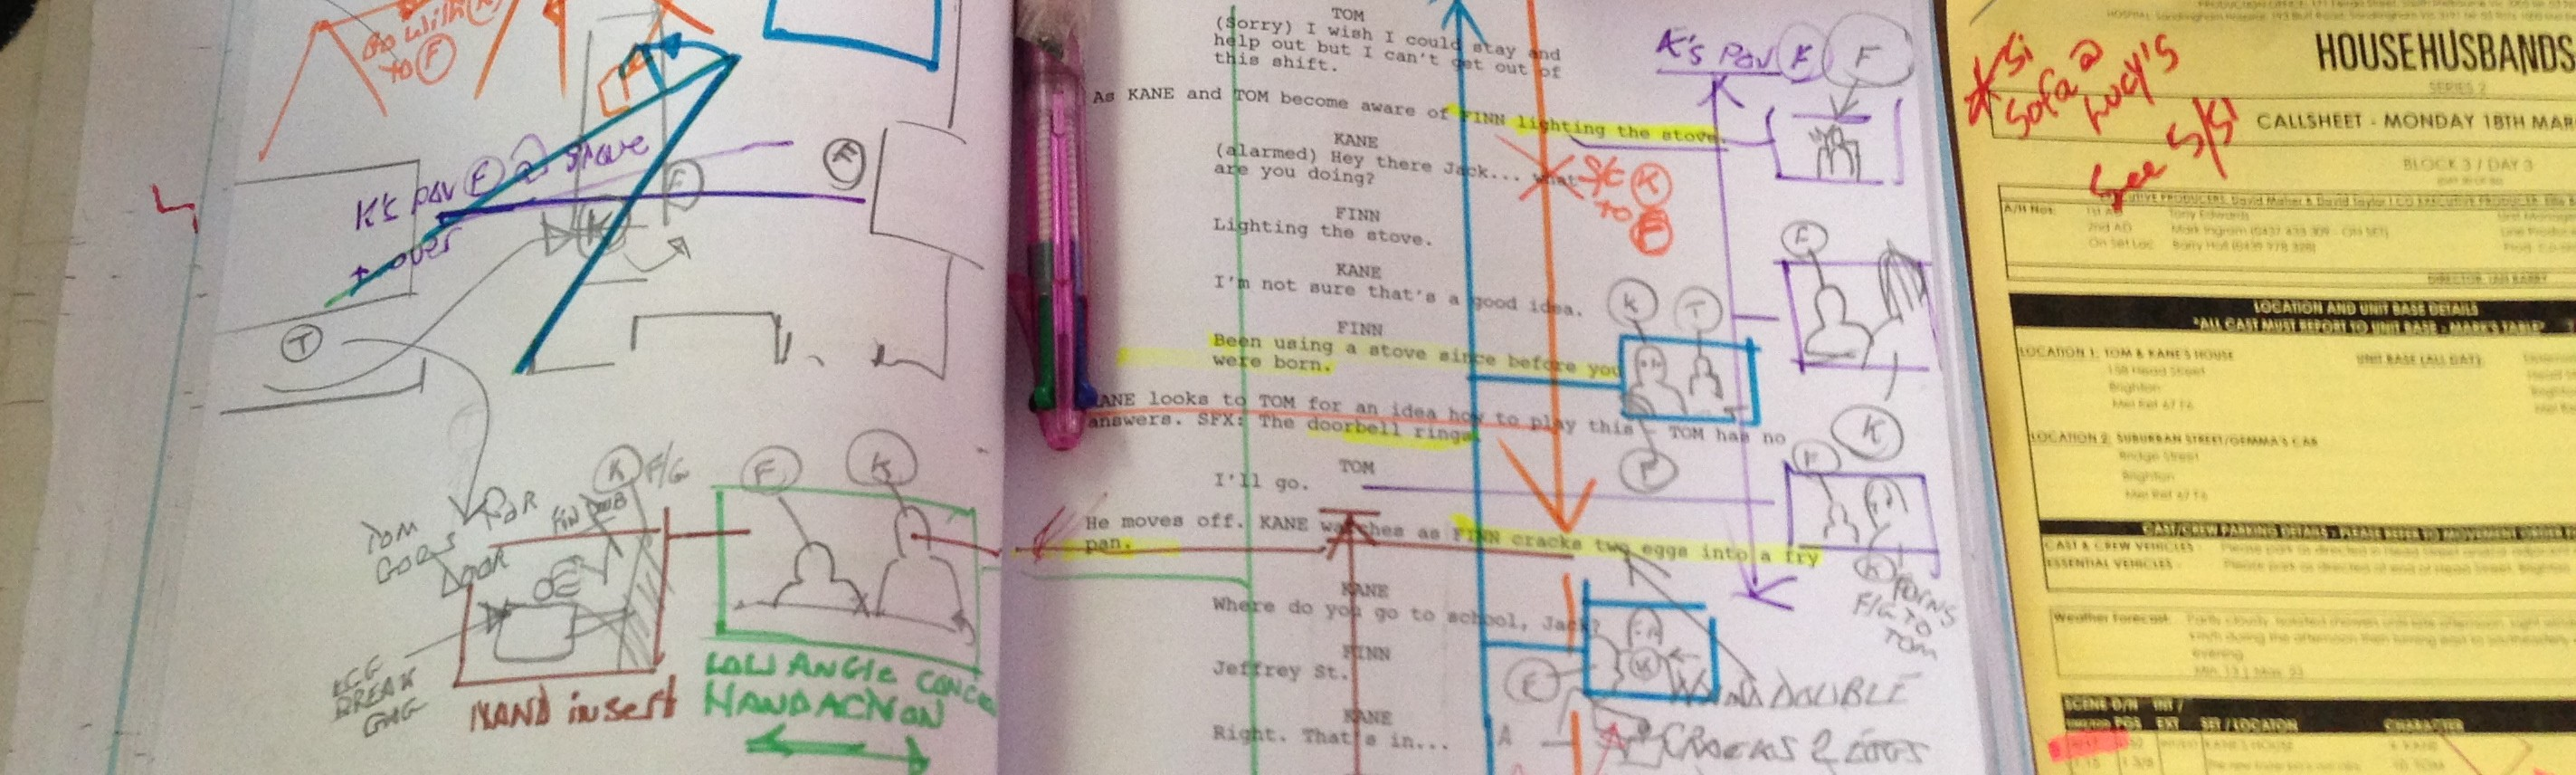
\includegraphics[width=0.8\textwidth]{figures/script_annotations.jpg}
\caption{Annotated script and notes on set of House Husbands~\cite{mskemosabi2013}}
\label{fig:script-notes}
\end{figure}

\subsection{From the Perspective of Script Supervisors}

Script supervisors enter the production pipeline 4–8 weeks before principal photography, conducting comprehensive script breakdowns that identify continuity elements, perform timing analysis, and create department-specific documentation. This pre-production phase produces the continuity master reference detailing costume changes, prop states, and temporal progressions across the narrative timeline. During filming, script supervisors arrive 30–60 minutes before crew call to coordinate daily continuity requirements. Positioned in video village, they document every take with technical camera data, timing information, and continuity observations whilst generating three essential documents: lined scripts showing coverage patterns, editor's logs detailing each take, and daily progress reports distributed within two hours of wrap.

Post-production responsibilities commence immediately after wrap, requiring 1–2 weeks to compile the production book containing all continuity documentation, lined scripts, and editorial notes. Script supervisors then remain available for 4–6 weeks of consultancy, resolving continuity questions during editing and providing specifications for potential reshoots. Their formal responsibilities conclude upon delivery and acceptance of all materials by the post-production team, though complex productions may retain them throughout editing to ensure narrative coherence~\cite{wickens2015,kreativalchemy2024}.

\section{Computer-Vision Capabilities and Limitations}

\subsection{Object Detection}

Modern object-detection systems follow two main approaches. Single-stage detectors examine entire images in one pass to find objects, a good example of such is the YOLO (You Only Look Once) family. YOLOv11 represents one of the latest iterations, which introduces architectural improvements including C3k2 (Cross Stage Partial with kernel size 2) blocks, which enhance feature extraction whilst reducing computational load, and parallel spatial attention mechanisms that help the model focus on relevant image regions. YOLOv11 achieves 54.5\% mAP on the COCO dataset whilst maintaining inference speeds of 13.5 milliseconds, making it suitable for real-time applications~\cite{ultralytics2024}. Recent comparative studies demonstrate that the YOLO series consistently balances speed and accuracy across different hardware configurations, with newer versions showing significant improvements in detecting smaller objects, which can be critical for video analysis tasks~\cite{khanam2024}.

Two-stage detectors take a different approach by first identifying regions likely to contain objects, then classifying those regions. Meta's Detectron2 framework implements this methodology through a modular design supporting various backbone networks~\cite{lv2023}. When configured with Mask R-CNN and ResNet-50-FPN, Detectron2 achieves 41.0\% box AP and 37.1\% mask AP on COCO (Common Objects in Context), prioritising accuracy over speed. This framework has proven particularly effective in medical imaging applications, achieving 99.3\% accuracy in diabetic retinopathy lesion detection~\cite{premiumbeat2023}. The modular architecture allows researchers to adapt components for specific requirements, such as tracking objects across video frames or detecting partially occluded items.

The choice between architectures depends on application requirements. Single-stage detectors excel in scenarios demanding immediate response, for example, autonomous vehicles require sub-20ms detection for safe navigation. Two-stage detectors are more suitable for applications that allow longer processing times, such as medical diagnosis or forensic video analysis where accuracy outweighs speed constraints. Recent developments in transformer-based models like DETR (DEtection TRansformer) begin to blur the traditional distinction between single-stage and two-stage detectors~\cite{carion2020}. However, traditional architectures remain dominant in production deployments due to their established performance characteristics and extensive optimisation for various hardware platforms.

\subsection{Semantic Understanding Gap}

The fundamental challenge lies not in detecting objects but understanding their narrative significance. Consider a coffee cup that appears half-full in one shot and empty in the next. Object detection easily identifies the cup's presence and even how full it is through segmentation. However, determining whether this change represents a continuity error (cup state changed incorrectly), intentional storytelling (character drank between shots) or an acceptable variation (minimal story impact) through semantic reasoning is beyond current computational capabilities. Nevertheless, the rapid advancement of Multimodal Large Language Models (MLLMs) promises to enable accurate image-to-text analysis. These models are already being deployed in complex applications, including semantic correction within text-to-image diffusion systems~\cite{tan2020}. At present, however, such models exhibit limitations in spatial reasoning, object recognition, numerical accuracy, and fine detail perception.

\subsection{Applicable Techniques}

Despite limitations in semantic understanding, several computer vision techniques show particular promise for continuity detection in film production:

Co-attention mechanisms for implicit correspondence: The COAM (Co-Attention Module) architecture enables automatic alignment between image pairs by computing cross-attention between feature maps. Each feature vector at location $(x_1, y_1)$ in the first image attends to all locations in the second image, creating spatially warped features that effectively register the images without explicit transformation computation. This approach achieves 60.7\% accuracy on change detection benchmarks whilst maintaining real-time performance at 6.37 seconds per frame pair~\cite{zhang2023}.

Siamese U-Net architecture with change detection heads: A dual-stream encoder processes image pairs simultaneously, extracting multi-scale features that are then cross-attended and decoded back to full resolution. The architecture concludes with a CenterNet detection head that produces bounding boxes around changed regions, effectively framing change detection as an object detection problem rather than pixel-wise segmentation. This design choice significantly reduces post-processing requirements whilst maintaining high localisation accuracy~\cite{zhang2023}.

Spatial Transformer Networks for geometric normalisation: STNs learn to predict homography parameters that transform cropped objects to canonical views, crucial for handling viewpoint variations in film shots. When applied to analogue clock reading, this alignment step improved recognition accuracy by 14.3\% on real-world data, demonstrating the importance of geometric normalisation even when objects appear at arbitrary angles or positions within the frame~\cite{ma2024}.

Time prediction through multi-class classification: Rather than regression-based approaches, treating time reading as a 720-way classification problem (12 hours × 60 minutes) provides more robust predictions. This discrete formulation naturally handles the circular nature of time and allows the network to learn common time patterns. Combined with pseudo-labelling techniques that exploit temporal uniformity in videos, this approach achieves 82.9\% accuracy without manual annotations~\cite{ma2024}.

PaddleOCR's DBNet for real-time text detection: The Differentiable Binarisation Network uses a learnable threshold map alongside the probability map to produce sharp text boundaries, achieving 80\% F-score at 8.7 FPS. Its modular design supports multiple recognition backends including CRNN and STAR-Net, making it adaptable for detecting various text elements within scenes~\cite{kuang2021}.

\section{Related Work Analysis}

\subsection{Pickup and Zisserman (2009)}

The sole directly relevant prior work, 'Automatic retrieval of visual continuity errors in movies'~\cite{pickup2009}, pioneered computational approaches to continuity detection. Their methodology:

\begin{itemize}
\item Detected shots using RGB histogram differences between consecutive frames
\item Matched shots from similar viewpoints using L1 histogram distances
\item Registered frame pairs using homography estimation with RANSAC
\item Excluded human regions using upper-body HOG detectors
\item Computed pixel-wise differences between registered frames
\item Ranked shots by the number of unexplained discrepancy pixels
\end{itemize}

Whilst Pickup and Zisserman's approach established foundational concepts for computational continuity detection, a few critical limitations prevent it from being applicable in production workflows. Most significantly, their system operates exclusively on fully edited sequences. It necessitates completed post-production before analysis even begins, which defeats the purpose of prevention-based continuity supervision. The evaluation methodology also presents concerns: whilst the paper successfully demonstrates retrieval of known errors from specific films, it lacks comprehensive accuracy metrics. Despite these limitations, the underlying design principles: shot matching through viewpoint similarity, geometric registration and human-aware exclusion zones retain conceptual validity. These techniques, reimplemented with modern architectures, could potentially address the real-time continuity monitoring challenge that the original work could not achieve.

\subsection{Adjacent Research Domains}

Computer Vision in Film Analysis: Schmidt et al.~\cite{schmidt2021} demonstrated that sampling films at one frame per second provides sufficient temporal resolution for narrative analysis. Their study applied object detection, emotion recognition, and demographic prediction to five canonical films, successfully identifying significant differences between genres and temporal patterns. This sampling rate aligns with our continuity detection requirements, as continuity errors persist across multiple seconds rather than occurring frame-by-frame. Their finding that object detection can reveal recurring motifs, such as clocks in Metropolis, suggests similar techniques could identify continuity-relevant objects across shots.

Sports Analytics and Tracking: Modern sports analytics employs transformer-based architectures for real-time multi-player tracking. SoccerNet-Tracking achieves 71.5\% HOTA (Higher Order Tracking Accuracy) with the ByteTrack algorithm across multiple camera views~\cite{cioppa2022}. The system tracks 22 players simultaneously at 25 fps. Recent basketball tracking systems incorporate deep learning models to predict player movements, with trajectory prediction achieving high accuracy for short-term horizons~\cite{hauri2022}. These advances demonstrate robust object tracking under rapid motion and occlusion. However, sports systems operate within constrained environments with fixed camera positions, advantages that might be unavailable in dynamic film sets.

Manufacturing Quality Control: Automated visual inspection systems have revolutionised defect detection in manufacturing, with state-of-the-art methods achieving detection rates exceeding 99\% for surface defects. Recent approaches like PatchCore achieve >99\% AUROC on the MVTec industrial anomaly detection dataset~\cite{farid2016}. Deep learning systems can identify defects as small as 0.02 mm² on high-speed production lines~\cite{wang2004}. This domain's emphasis on detecting subtle deviations from expected patterns directly parallels continuity error detection. Manufacturing systems excel at identifying 'what should not be there', precisely the challenge when attempting to detect misplaced props or costume changes between takes.

Autonomous Vehicle Perception: Current autonomous driving systems process visual data at unprecedented scales. Waymo's 5th generation perception stack utilises 5 LiDAR units and 29 cameras, processing millions of 3D points per second~\cite{waymo2020}. The Waymo Open Dataset demonstrates the scale of modern autonomous perception, containing over 12 million 3D bounding box annotations across diverse driving conditions~\cite{sun2020}. The domain's expertise in handling varying weather conditions, occlusions, and multi-object tracking provides methodological insights. Particularly relevant is the use of temporal fusion techniques that aggregate information across multiple frames to improve detection reliability. However, these computational capabilities far exceed film production requirements.

\section{Summary}

The background analysis reveals a complex problem at the intersection of cognitive science, film production and computer vision. Human limitations in sustained vigilance tasks create genuine need for automated assistance. Current production workflows provide integration opportunities in natural reset windows. Although computer vision has achieved remarkable capabilities, the semantic understanding required for continuity detection remains challenging. The absence of prior research, despite a clear industry niche, highlights both the difficulty and opportunity this problem presents.
\chapter{System Design and Architecture}
\label{ch:design}
\section{Requirements Analysis}
CAM-F's design emerged from systematic analysis of film production constraints, technical requirements and user needs. Rather than pursuing technical sophistication for its own sake, every design decision prioritised practical deployability and operational simplicity whilst maintaining the modularity needed for research advancement. Through extensive literature review of industry workflows, analysis of existing professional production tools, and investigation of documented continuity practices in film, we identified critical requirements that shaped the architectural decisions.
\subsection{Production Environment Constraints}
Film sets present unique deployment challenges absent from typical video-capture software environments. Keeping footage secure and unreleased before official distribution is essential for productions to maintain commercial value. Systems must operate fully offline to ensure full safety whilst maintaining functionality. This might eventually limit the capabilities of specialised detectors that could need access to external tools. However, the project's goals necessitate network isolation, which ensures deployment-ready application and, at the same time, showcases feasibility even in these limited conditions. 
Productions cannot dedicate high-end servers to continuity detection. The system must run on script supervisors' portable hardware that travels between locations and allows for minimal setup costs. Operational simplicity is another key aspect of design requirements. Set personnel focus on filmmaking, not IT administration. Complex deployment procedures or ongoing maintenance requirements would prevent seamless integration into existing workflows. With hundreds of crew members depending on production and tight schedules, reliability of the system is essential. Failures cannot interrupt filming, so graceful degradation takes priority over feature completeness.
\subsection{Performance Requirements}
Temporal analysis of production workflows shows specific performance targets. Reset windows between takes define maximum acceptable processing time. It varies enormously based on shot complexity, crew size, equipment requirements, location constraints and directorial style. Nevertheless, we can estimate the average distribution:
68\% of resets: 2–5 minutes
24\% of resets: 5–15 minutes
8\% of resets: >15 minutes
To capture the majority of opportunities to prevent any anomaly, processing must complete within 5 minutes after the take's cut. For example, given average take lengths of 45 seconds, this requires processing 45 seconds of footage within 345 seconds (including the take length), or 7.6× real-time minimum. This makes time to detect the essential metric requirement for the system.
Another essential requirement is the detection accuracy, which determines the system's trustworthiness and practical potential. Unfortunately, due to the lack of published studies and error rate statistics it is hard to set a distinctive benchmarking for accuracy. Based on vigilance task research demonstrating 10-30\% performance degradation in sustained attention tasks [9], we conservatively estimate human detection accuracy at 75-80\% over typical 10-14 hour production days, accounting for the mitigating effects of professional tools and techniques employed by script supervisors. This provides a baseline against which automated detection performance can be measured.
Important to note that missing a continuity anomaly that reaches final edit proves far more expensive than investigating a false alarm during principal photography. Which makes the false negatives (missed errors) far more relevant than false positives (incorrect alerts).
\subsection{Other Non-Quantifiable Requirements}
Detector extensibility: Different productions face varying continuity challenges. Since covering everything is not feasible, the framework must support development of specialised detectors addressing different error types, from simple prop tracking to complex semantic analysis, without requiring core system modifications.
Result transparency: Detection outputs must provide clear explanations and visual evidence for flagged issues. Script supervisors need to quickly understand why the system flagged a potential error and make informed decisions about its validity.
Workflow integration: The system must integrate seamlessly with existing production practices without disrupting established routines. Script supervisors should access detection results through familiar interfaces that complement, rather than replace, current tools.
Long-term data management: Extended productions accumulate thousands of takes across multiple shooting days. The system must store all captured frames, detection results and associated notes in an organised, searchable structure that enables rapid retrieval of any historical reference. 
\section{Architecture Overview}
CAM-F implements a hybrid architecture combining a monolithic backend with process-isolated detector plugins. The system consists of four primary components: a single Python process hosting all core services, a Tauri-wrapped React frontend, isolated detector processes managed through multiprocessing, and a hierarchical storage system mapped to film production workflows.
Figure 3.1 illustrates the system architecture. The backend process contains Storage, Capture, Detector Framework, and Export services running in shared memory. These services communicate through direct method calls, eliminating serialisation overhead. The API Gateway runs in a separate thread within the same process, providing REST endpoints and SSE (Server-Sent Events) channels for frontend communication. Each detector executes in a sandboxed subprocess with enforced resource limits and restricted filesystem access.

\begin{figure}[h]
\centering
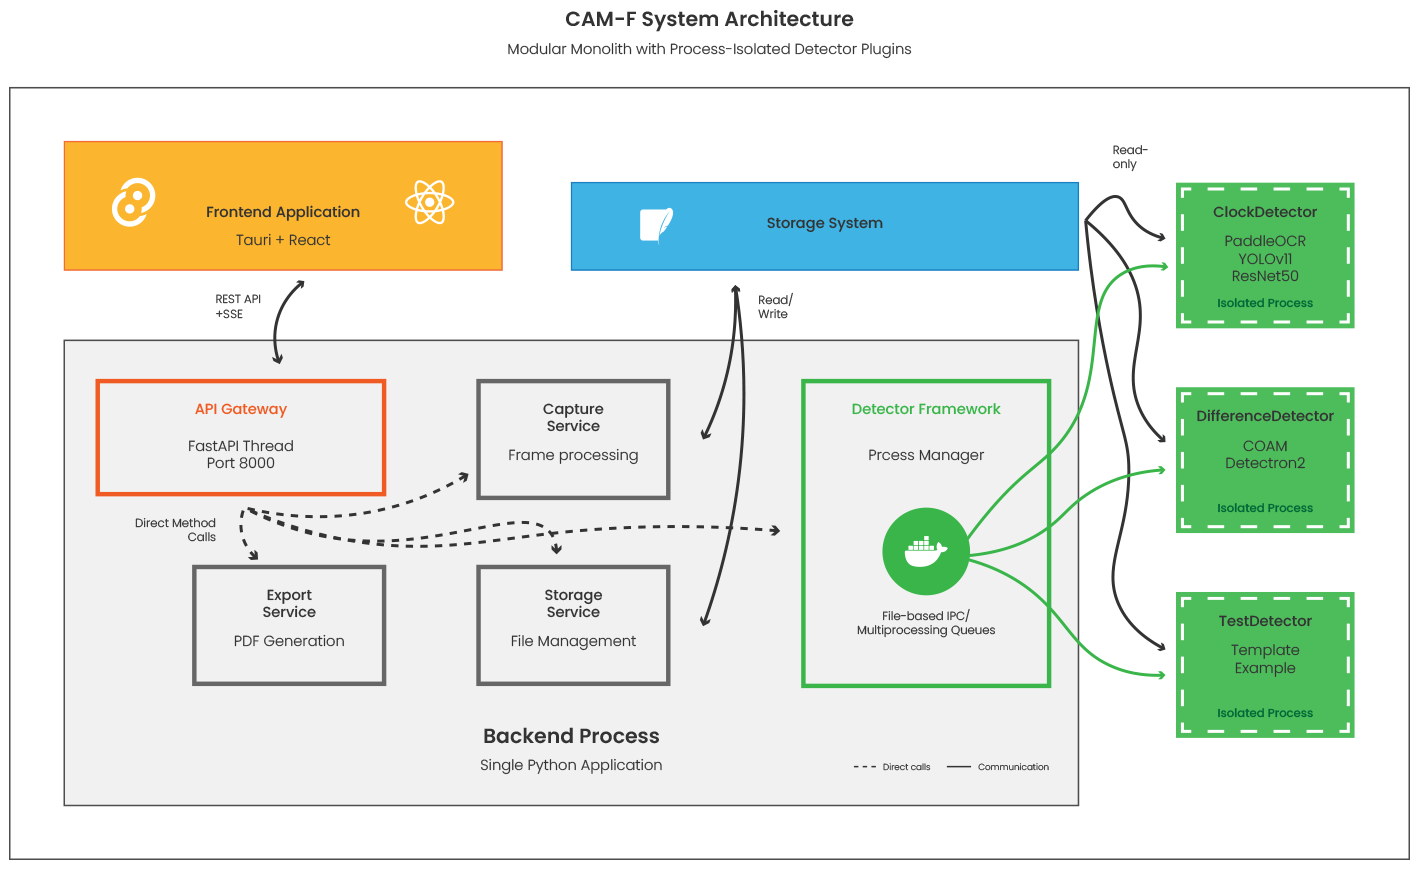
\includegraphics[width=0.9\textwidth]{figures/Architecture.png}
\caption{CAM-F System Architecture showing monolithic backend with sandboxed detector plugins. Services communicate via direct method calls while detectors use JSON-RPC over stdin/stdout.}
\label{fig:architecture}
\end{figure}
\section{Key Design Decisions}
\subsection{Implementation Platforms}
Python serves as CAM-F's backend language due to its dominance in computer vision deployment. All major object detection frameworks, including YOLOv11 and Detectron2 used in our detector implementations, provide Python APIs exclusively. OpenCV's Python bindings enable efficient frame capture and preprocessing without performance penalties through optimised C++ implementations underneath. The multiprocessing module provides process isolation primitives essential for detector sandboxing, handling IPC and lifecycle management through platform-agnostic abstractions.
React powers the frontend to handle real-time UI updates from continuous frame capture. Its virtual DOM (Document Object Model) reconciliation minimises rendering overhead when updating frame previews, helpful for resource-constrained laptops common on film sets. Zustand manages application state with small footprint, whilst TanStack Query handles API communication with built-in retry logic and request deduplication. This technology stack prioritises ecosystem compatibility and production deployment requirements over theoretical performance optimisations, ensuring CAM-F integrates with existing computer vision research whilst remaining deployable by non-technical users.
\subsection{Technology Stack}
FastAPI: The backend uses FastAPI to handle REST endpoints and SSE channels. FastAPI's asynchronous request handling enables concurrent processing of capture commands, storage queries and detector status updates without blocking. Built-in error recovery middleware ensures graceful handling of detector failures without affecting other system components. We also use the framework's automatic OpenAPI schema to generate interactive documentation. It allows developers to test endpoints directly, which supports community-driven development.
Docker SDK: Each detector execution is managed in its own isolated container. When a detector processes frames, the framework spawns a container with comprehensive security controls:
Flexible resource allocation: No default limits on memory, CPU or processes allowing intensive CV/ML workloads to utilise available resources (configurable). 
Filesystem isolation: Read-only root filesystem with writable workspace areas for computation
Network isolation: Disabled networking prevents footage exfiltration
System call filtering: Custom \verb|seccomp| profiles restrict dangerous operations
AppArmor integration: Additional MAC (Mandatory Access Control) layer when available
The SDK's Python interface enables programmatic container lifecycle management, from image building during detector installation to automatic cleanup after processing completion. It is not only essential for safety measures, but also to allow detectors the freedom and control over the environments they need to set up for computation.
SQLite: The storage service uses SQLite as an embedded database for metadata management. ACID-compliant transactions ensure data integrity during unexpected shutdowns. The data model directly maps to production hierarchy: projects, scenes, angles, takes, and frames.
Tauri: The frontend wraps React using Tauri 1.5, which currently only supports native desktop applications for Windows, but can be easily extended to other OS. Tauri produces much smaller executables than similar technologies by leveraging system WebView components rather than bundling browser engines. The framework's secure IPC bridge also contributes to security measures by restricting filesystem access to designated directories.
Server-Sent Events (SSE): Real-time updates flow from backend to frontend through SSE channels. The unidirectional nature matches CAM-F's communication pattern where the server broadcasts capture progress and detector results. SSE's automatic reconnection with exponential backoff handles any interruptions. Event queues limited to 100 messages prevent memory exhaustion whilst maintaining UI responsiveness.
\subsection{Storage Strategy}
The storage architecture mirrors the production hierarchy. CAM-F organises footage by project, scene, angle, and take as shown in Figure 3.2.

\begin{figure}[h]
\centering
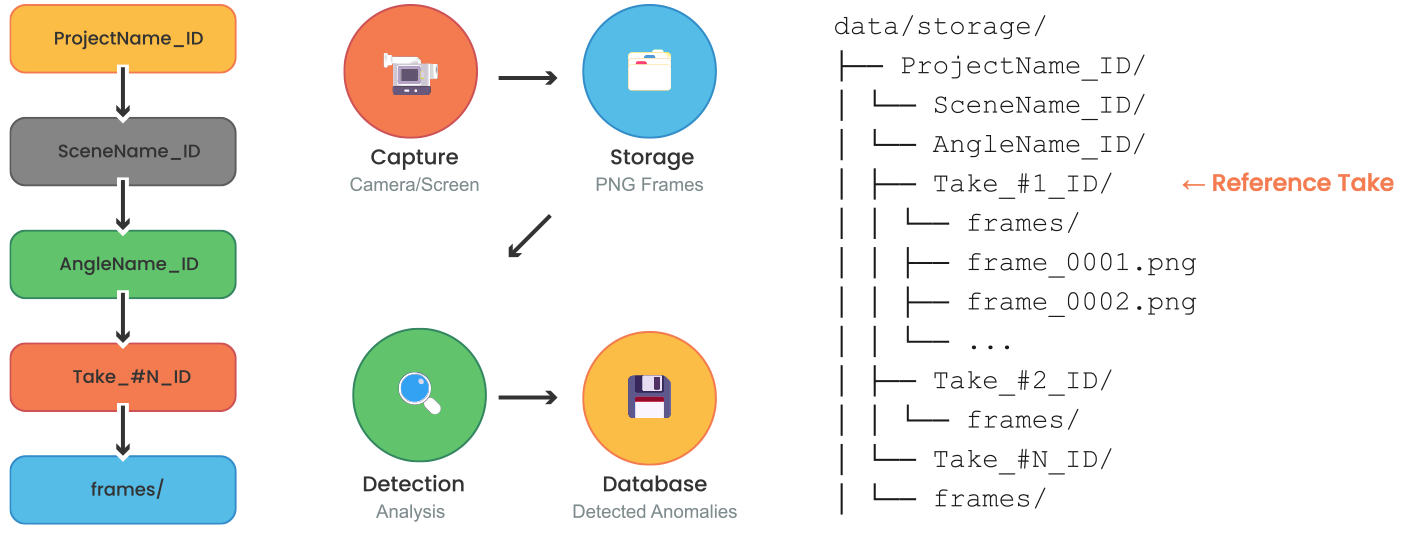
\includegraphics[width=0.7\textwidth]{figures/storage.png}
\caption{Hierarchical storage structure mirroring film production workflow. Each level maps to production concepts with unique IDs preventing naming conflicts.}
\label{fig:storage}
\end{figure}

Individual frames are stored as PNG files enabling random access for detector processing. Scene and custom detector configurations attach at the scene level, as it's being initialised, and are applied across all its descendants. We also automatically establish reference take as baseline for continuity. The first take of each angle automatically becomes the reference unless manually overridden. Subsequent takes compare against this reference for anomaly detection.
Continuity errors detected by the framework are stored in the database where they can be quickly searched and filtered. The system tracks individual detections on each frame (confidence scores, locations, which detector found them), false positives marked by the production team and errors that span multiple frames. Custom result deduplication algorithm prevents alert fatigue from continuous errors. The system groups spatially and temporally proximate detections, presenting them as single issues rather than flooding supervisors with redundant notifications.
\section{Core Framework Components}
\subsection{Real-time Monitoring Pipeline}
The monitoring pipeline implements push-based stream processing, a fundamental design choice that influences the entire system architecture. When the capture service acquires a frame, it immediately pushes the data through the processing pipeline rather than allowing detectors to pull frames on demand. This approach optimises for minimal latency over maximum throughput, reflecting production requirements where immediate feedback proves more valuable than processing efficiency.
Frame data flows through the system using storage as the communication medium rather than memory or network transfer. The capture service writes each frame once to persistent storage, after which multiple detectors read the frame data independently. This pattern appears inefficient compared to in-memory passing, yet provides several critical advantages:
Single source of truth: Frame data exists in one authoritative location
Natural audit trail: All captured frames remain available for review
Reduced memory pressure: No frame duplication across process boundaries
Simplified recovery: System restart automatically recovers all persisted frames
The pipeline adopts a shared-nothing architecture where each detector processes frames independently without inter-detector communication or shared state. This design eliminates coordination overhead and prevents cascading failures, though it prevents any collaborative detection strategies where multiple detectors might share intermediate results. The simplicity and reliability benefits outweigh the potential advantages of multi-detector cooperation.
\subsection{Frontend Event Distribution}
The event system uses SSE for unidirectional server-to-client communication. This design ensures the backend remains the sole authority for state changes. Clients request modifications through REST APIs but cannot directly alter system state, preventing synchronisation conflicts common in bidirectional systems. Events transmit complete state rather than change notifications. Network interruptions become trivial to handle as reconnecting clients receive current state immediately. Internal service communication differs fundamentally from external UI updates. Backend services communicate through direct method calls, ensuring reliable and ordered message delivery. UI clients receive events through SSE with best-effort delivery. When clients fall behind, the system drops older events to maintain real-time relevance. This separation provides appropriate guarantees for each communication type without unnecessary complexity.
The architecture remains deliberately simple. Rather than implementing complex event sourcing or message queuing systems, CAM-F uses straightforward patterns. Multiple clients can subscribe to event streams without registration overhead. Commands and queries follow separate paths (REST for commands, SSE for updates) but share the same simple state model.
\subsection{Security Measures}
Catering to deployment ready system with proper protections while trying to promote researchers to apply various methodologies to continuity creates a challenging dilemma. Since this project aims to put foundation for further work, it's crucial to convey all the relevant aspects of the field. All these limitations can be easily configured and disabled for the sake of freedom in development. However, setting a premise where such protections are overlooked promotes poor legal and ethical practices. 
Every detector executes within a Docker container configured for high level of isolation. Network access is completely eliminated through \verb|network_mode: "none"|, making data exfiltration impossible regardless of the detector's code. The root filesystem operates in read-only mode, with write permissions limited to \verb|/tmp| (1GB) and \verb|/dev/shm| (2GB). These temporary spaces accommodate computational needs whilst preventing persistent data storage.
Beyond filesystem restrictions, the containers drop all Linux capabilities via \verb|cap_drop: ["ALL"]| and employ Seccomp profiles to filter system calls. This kernel-level filtering blocks potentially dangerous operations before they execute. Additionally, detectors run under dedicated non-root users without shell access, creating multiple barriers against system compromise.
The system provides several features:
Automatic GPU passthrough for hardware acceleration
2GB shared memory allocation for PyTorch \texttt{DataLoader} operations
Pre-configured parallel processing environment variables
Model cache directories to avoid repeated downloads
Frame data reaches detectors through filesystem paths passed via JSON-RPC messages. Rather than serialising image data, which would've been more secure, the framework sends only the file paths where frames are stored (see Figure 3.3). This design eliminates serialisation overhead while the security is maintained by process isolation. The detectors cannot access the primary storage hierarchy or other system resources beyond its allocated workspace.

\begin{figure}[h]
\centering
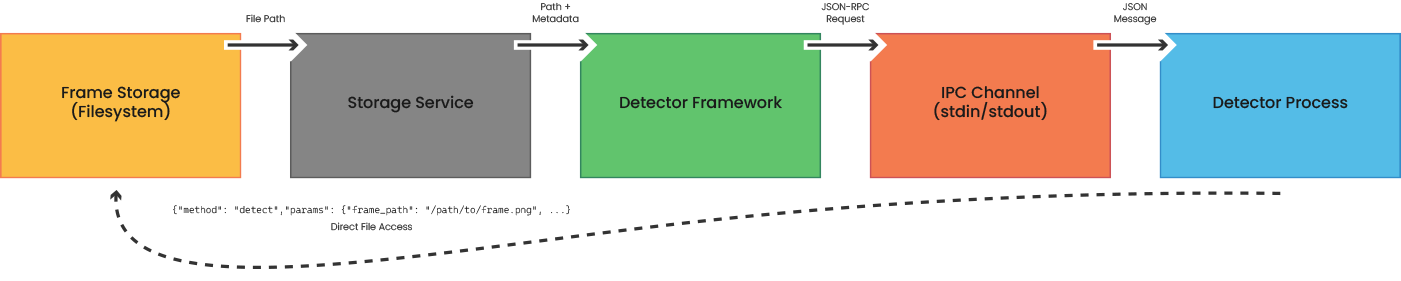
\includegraphics[width=0.8\textwidth]{figures/comms flow.png}
\caption{Communication flow between framework and sandboxed detectors. JSON-RPC messages contain frame paths rather than image data, reducing serialisation overhead whilst maintaining security through process isolation.}
\label{fig:comms-flow}
\end{figure} 
\subsection{Reliability Practices}
During the workload of monitoring anomalies, the key long-term component is consistent frame capture. CAM-F prioritises operational continuity through sophisticated failure handling that keeps it running regardless of various failures. The capture service operates independently from detector processing. Frames are queued asynchronously for detection, ensuring capture continues uninterrupted even during complete detector failures. Detector failures trigger progressive recovery through five strategies:
Immediate restart for transient failures
Exponential backoff (1-60 seconds) for recurring issues
Frame skipping for consistently problematic frames
Fallback mode with reduced processing quality
Automatic disabling after excessive consecutive failures
The recovery manager analyses failure patterns including consecutive failures, time-based clustering and frame-specific issues used in appropriate strategy selection. Recovery state persists to \texttt{detector\_recovery\_state.json}, preserving learned failure patterns across system restarts.
\section{Detector Design}
The detector architecture defines how individual detection algorithms integrate with CAM-F. Each detector operates as a self-contained unit that analyses frame pairs for specific continuity errors. This modular design allows researchers to develop specialised detectors without understanding the framework's internal complexity.
\subsection{Manifest Driven Architecture}
Every detector includes a \texttt{detector.json} manifest file that declares its capabilities and requirements. This manifest specifies whether the detector needs GPU access, how much memory it requires, and what configuration options users can adjust. The framework reads these declarations before running any detector code, preventing incompatible detectors from installing on systems that cannot support them. Configuration schemas automatically generate user interfaces, eliminating manual UI development. A few of the other configurations are there solely for inspiration and showcase of potential use-case scenarios. For example, memory declarations can allow the system to calculate whether multiple detectors can run simultaneously or not, notifying the user of computational limitations.
This design differs from traditional plugin systems that discover capabilities at runtime. By requiring explicit declarations, CAM-F provides transparency about resource usage. Script supervisors can understand why certain detectors need specific hardware or take longer to process frames. The manifest becomes a clear specification of what each detector does and what it needs to function.
\subsection{Three-Phase Execution Model}
Detectors follow three distinct phases: initialization, processing, and cleanup. This structure reflects common patterns in computer vision workflows where model loading represents a significant one-time cost.
During initialization, detectors load neural network weights and allocate GPU memory. This phase runs once when a detector activates, with costs amortised across thousands of subsequent frames. The framework enforces a configurable timeout (default 30 seconds) to prevent stuck detectors from blocking the system.
The processing phase handles frame pair analysis. Each invocation receives current and reference frames as NumPy arrays, along with metadata about take numbers and timestamps. Detectors analyse these inputs and return a list of detected errors. While the architecture encourages stateless processing for deterministic results, detectors can maintain internal state within their container lifetime if needed.
Cleanup ensures proper resource release when detectors deactivate. GPU memory must be freed and temporary files deleted. The framework monitors this phase with a configurable timeout, forcibly terminating detectors that fail to clean up properly.
\subsection{Error Reporting Structure}
Detector outputs follow a standardised format designed for production use. Each error report includes five components:
Error type: A categorical classification like \texttt{"prop\_missing"} or \texttt{"wardrobe\_change"} that enables filtering and statistical analysis.
Confidence score: A probability between 0.0 and 1.0 indicating detection certainty. Productions can adjust thresholds based on their tolerance for false positives.
Spatial location: A bounding box with x, y, width, and height coordinates for visual overlay on frames.
Description: Plain language explanation written for script supervisors, not engineers.
Details: Additional structured data like object classes or colour values for further processing.
This format is based on how script supervisors process information during production. Technical metrics alone are insufficient when they need to make rapid decisions. The combination of visual location, confidence score, and human-readable description provides the context needed for quick assessment.
\subsection{Communication Protocol}
The framework communicates with detectors through standard input and output streams using JSON-RPC messages. Each detector runs as a separate process, receiving commands through \texttt{stdin} and sending results through \texttt{stdout}. This approach provides real-time communication without the delays inherent in filesystem-based message passing. The choice of \texttt{stdin}/\texttt{stdout} ensures any programming language can create a detector by simply reading and writing text streams.
The protocol separates control messages from frame data to maintain efficiency. JSON messages contain only commands and metadata, while actual frames remain in filesystem storage. When the framework needs a detector to analyse frames, it sends paths rather than image data. This design keeps messages small and allows the operating system to handle efficient file access through memory mapping. A configurable timeout on each message exchange prevents failed detectors from blocking the entire system.

Python's multiprocessing queues manage the underlying communication complexity. Rather than implementing custom inter-process communication, the framework uses proven standard library components. This reduces potential bugs and simplifies maintenance whilst providing reliable message delivery between the framework and detector processes. The architecture trades a small amount of theoretical performance for substantial improvements in stability and overall comprehension.
\subsection{Development Experience}
The framework provides a \texttt{BaseDetector} class that abstracts away all communication and protocol complexity. Developers inherit from this class and implement only the detection logic, typically just adjusting the \texttt{process\_frame\_pair} method. The base class handles JSON-RPC parsing, timeout management, frame loading, and error serialisation automatically. This abstraction transforms what could be a complex distributed system into a simple Python class with minimal boilerplate.
Testing detectors locally requires no Docker installation. The framework supports dual-mode execution where detectors run as standard Python processes during development. Virtual environments provide dependency isolation without container overhead. Developers can attach debuggers, inspect variables, and iterate quickly on their algorithms. When ready for deployment, the same code runs in Docker containers without modification. This flexibility recognises that forcing containerisation during development would significantly slow the refinement.
The standardised project structure simplifies packaging and distribution. A detector requires only three files: the Python implementation, \texttt{requirements.txt} for dependencies, and the manifest. Developers package these as a ZIP archive for distribution. The framework handles all complexity of building Docker images, installing dependencies, and registering detectors. This minimal structure allows computer vision researchers to share their work without learning containerisation, package management, or deployment procedures.
\section{Production Workflow Integration}
Standalone System: CAM-F operates independently alongside script supervisors' current workflow rather than replacing established practices. It avoids the complexity of integrating with ScriptE, MovieSlate, and other proprietary studio systems. Each of these tools stores data differently and updates frequently. To mitigate added overhead of managing another system CAM-F produces universal formats for the outputs that work with any production workflow.
Hierarchical Export System: The export architecture allows reports at any production level. A take export contains just that take's errors and annotations. Scene exports include all takes organised by camera angles, while project exports encompass the entire production hierarchy. This granular control enables efficient knowledge distribution across departments. Script supervisors might export individual takes for immediate review, while post-production coordinators need complete scene documentation.
Automatic Reference Take Management: The first successful take at each camera angle becomes the continuity baseline, matching standard production practice. Subsequent takes compare against this reference automatically. Supervisors can override the selection if needed.
Scene-Based Configuration: Detector settings apply uniformly at the scene level. All angles and takes within a scene share the same configuration, reflecting how productions maintain consistent continuity standards throughout related shots. A car chase scene enables motion-based detectors while a dialogue scene prioritises prop and wardrobe checks. This flat configuration model eliminates complexity while serving most production needs.
\chapter{Implementation}

\section{Overview}
Building CAM-F from conception to deployment required integrating multiple computer vision technologies, real-time processing systems and some optimisation/reliability mechanisms. The implementation spans several interconnected components that work together to provide real-time continuity monitoring during active film production:

\textbf{Core Framework}: The monolithic backend provides a unified Python application managing all system operations. Built with FastAPI, it orchestrates frame capture, detector execution, and result aggregation. The system provides REST endpoints and Server-Sent Events for frontend communication. Only detector plugins execute in separate sandboxed processes.

\textbf{Detector Plugins}: Two proof-of-concept detectors demonstrate the framework's monitoring capabilities:
\begin{itemize}
\item \textbf{ClockDetector}: Combines YOLOv11 object detection with ResNet50-based time prediction model for analog clocks and PaddleOCR for digital displays.
\item \textbf{DifferenceDetector}: Implements co-attention networks for spatial change detection with specialised masking ignoring unnecessary motion anomalies.
\end{itemize}

\textbf{Production Optimisations}: To improve various performance metrics we implement error deduplication, multi-tier result caching with memory/disk persistence and failure recovery. We allow flexible control over the quality and resolution of an input along with capture rate. Monitoring using capture provides feed from various sources and for video upload we enable batch processing. Detectors are working in parallel with each other as frame pairs are pushed to their internal queues by the system.

On top of implementing a near deployment-ready application for script supervisors, we also incorporate a variety of small developer-friendly features that assist in research, building and debugging of new detectors. Although we aim for a high-quality final product, the main purpose of this implementation still remains within the scope of practical assessment and establishing a basic foundation for further research.

\section{Monitoring Pipeline}

\subsection{Capture to Storage}
The frame processing pipeline represents the core of CAM-F's operation. When monitoring begins, the capture service acquires frames from connected cameras or screen capture sources. Using OpenCV's platform-agnostic capture interface, the system supports multiple input sources: USB cameras, built-in webcams, DirectShow devices on Windows, V4L2 devices on Linux, screen and application capture. Regardless of source, frames arrive as NumPy arrays in BGR colour space, then undergo immediate serialisation to PNG format.

PNG's lossless compression preserves the visual fidelity while significantly decreasing file size. Instead of distributing BGR arrays to detectors and serialising them every time, we process and write it once. And then through file path communication we allow access to each PNG frame, which after the first read is cached by the OS. 

The storage service writes each frame to a hierarchical directory structure that mirrors production organisation. A frame captured during "Scene 4, Angle 2, Take 5" is located at a predictable path within the project file system: "data/storage/ProjectName\_1/Scene4\_2/Angle2\_3/Take5\_4/frames/frame\_000001.png". To maintain relationships with the database, while keeping customisation and readability, we utilise the ID-tagged naming convention \{Name\}\_\{DatabaseID\}.

\begin{figure}[h]
\centering
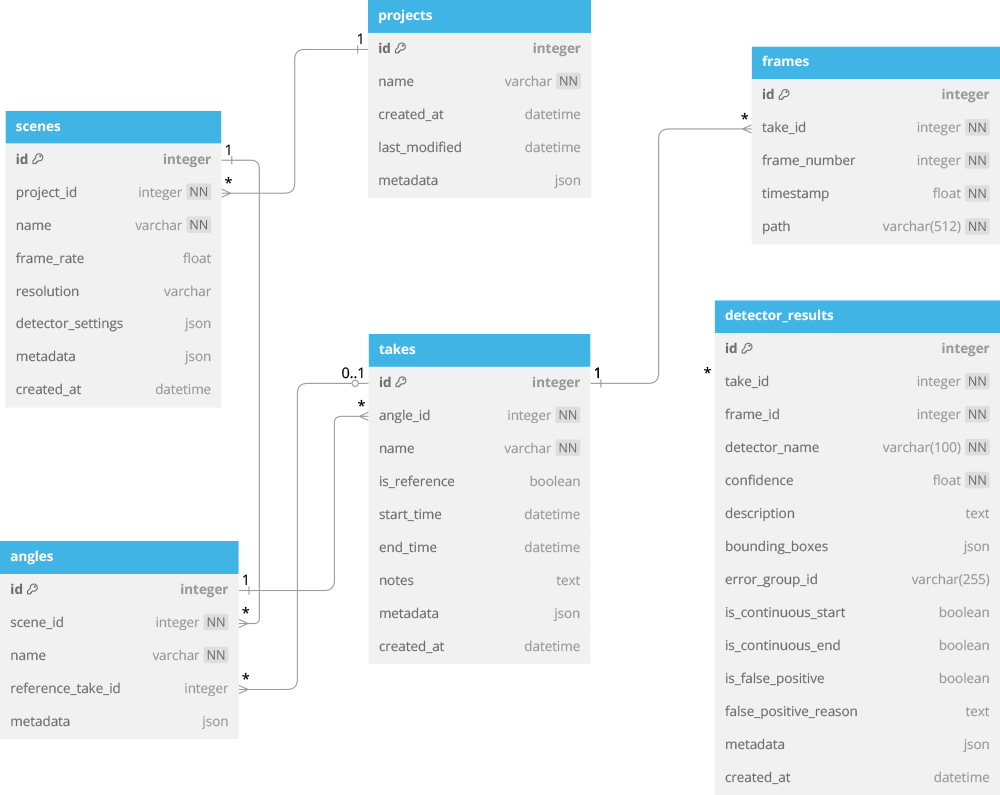
\includegraphics[width=0.9\textwidth]{figures/database.png}
\caption{Database schema showing relationships between projects, scenes, angles, takes, frames and detection results. The hierarchical structure enables efficient queries while foreign key constraints maintain referential integrity.}
\label{fig:database-relationships}
\end{figure}

\subsection{Reference Management}
Continuity detection fundamentally involves comparison. The goal is to identify what changed between the reference state and current state. The system automatically designates the first successful take of each scene angle as the reference baseline. This matches standard production practice where initial takes establish the continuity foundation, and the notes along with the images that the supervisor aggregates are used as reference.

We do not implement any sort of frame alignment or restrict specific timings to match total frame count for subsequent capture. While the frame rate is fixed for the entire scene configuration, due to the manual nature of capture controls, each take may still differentiatie by starting slightly earlier or being delayed. To mitigate the difference in frame counts, we stop processing at the lowest between the two. Depending on frame rate, temporal inconsistency in the action within the reference and current take has minor or no effect whatsoever on the detector and its accuracy. The implemented proof-of-concept detectors integrate the layer that deals with action interpretations.

At any point during principal photography, script supervisors may overwrite the reference take, of which each angle in a scene can only have one to avoid complexity. This change doesn't trigger the whole system overload, instead each take keeps the results from the latest processing session. However, at any point, the supervisor may redo the detection against a newly assigned reference. The system also allows user to select a specific take from any angle in the scene for a single instance processing.

\subsection{Frame Distribution}
Frame distribution to detectors employs a push-based model prioritising latency over throughput. When a new frame arrives, the framework immediately notifies all active detectors rather than waiting for detectors to pull for work. This design reflects production reality where immediate feedback during short reset windows proves more valuable than processing efficiency.

The distribution mechanism handles detector heterogeneity gracefully. Some detectors might opt to process frames individually, for example, a particular configuration of our ClockDetector examines current frames only. Others require frame pairs at all times. The framework abstracts these differences, providing each detector with appropriate frame sets based on their declared requirements in their manifest.

Queue management prevents system overload when detectors cannot maintain capture pace. Each detector receives an independent queue with configurable depth limits. When queues approach capacity, the framework begins selective frame dropping using importance-based prioritisation. First and last frames of each take receive highest priority as continuity errors frequently occur at shot boundaries. Middle frames are dropped first when processing falls behind.

\subsection{Result Aggregation}
Result aggregation begins immediately as detections arrive. The framework performs intelligent deduplication to reduce noise from persistent errors. Each detector's results are processed separately; when a detector identifies an anomaly, the system checks if it represents a continuation of the same one from previous frames. Spatial clustering uses two methods: bounding box overlap (IoU > 0.5) and center distance (<100 pixels) to determine if detections in consecutive frames represent the same underlying issue. This temporal-spatial grouping means a clock misalignment detected across multiple frames by a single detector appears as one continuous error rather than flooding supervisors with frame-by-frame alerts. However, to preserve unique findings and perspectives of each specialised detector the system deliberately maintains separation between them.

The bounding boxes, that describe the areas of concern within each frame, are stored as JSON metadata alongside the detection results. The system maintains complete data integrity - original frames remain untouched while detection overlays and annotations are stored separately in the database. On request these bounding boxes are generated as an overlay on top of the frames.

To assist research and development of new detectors we implement a small false positive management to handle cases where detectors are wrong. When supervisors identify a false positive, they can mark it directly in the interface with a reason. This allows for integration of supervised learning for specialised detectors. The reason for this integration was not just a mere gimmick for developers, it was important to allow script supervisors to have control over the results that they export. This way, they don't have to manually annotate exports with the wrong detections produced during monitoring.

The export system transforms aggregated results into production-ready documentation. PDF reports are generated with customisable notes from script supervisor, which can be edited within the UI, and a separate error section that provides a detailed frame-by-frame breakdown of all detections without duplications.

\section{ClockDetector}

\subsection{Detector Overview}
ClockDetector identifies temporal inconsistencies in film production by detecting and reading both analog and digital clocks. The implementation addresses two distinct challenges: interpreting analog clock faces with varying designs and perspectives, and recognising digital time displays across different device types. The detector employs separate processing pipelines for each clock type, unified through a common error reporting framework. When time discrepancies exceed configurable thresholds, the detector generates detailed continuity errors. 

\subsection{Analog Clocks}
Initial attempts to read analog clocks through geometric analysis showed undermining results. Direct calculation of hand angles failed to accommodate the diversity of clock designs, perspective distortions, and visual artifacts. When attempting to accurately detect the clock hands and calculate the displayed time, external visual factors significantly impacted performance, which led to very low accuracies below 40\%.

This limitation was clearly not practical for accurate real-time monitoring. After extensive literature review on time reading we decided to adopt the approach presented by Yang et al. in "It's About Time: Analog Clock Reading in the Wild" [23]. Their research demonstrates that analog clock reading benefits from a learning-based approach rather than geometric computation.

\begin{figure}[h]
\centering
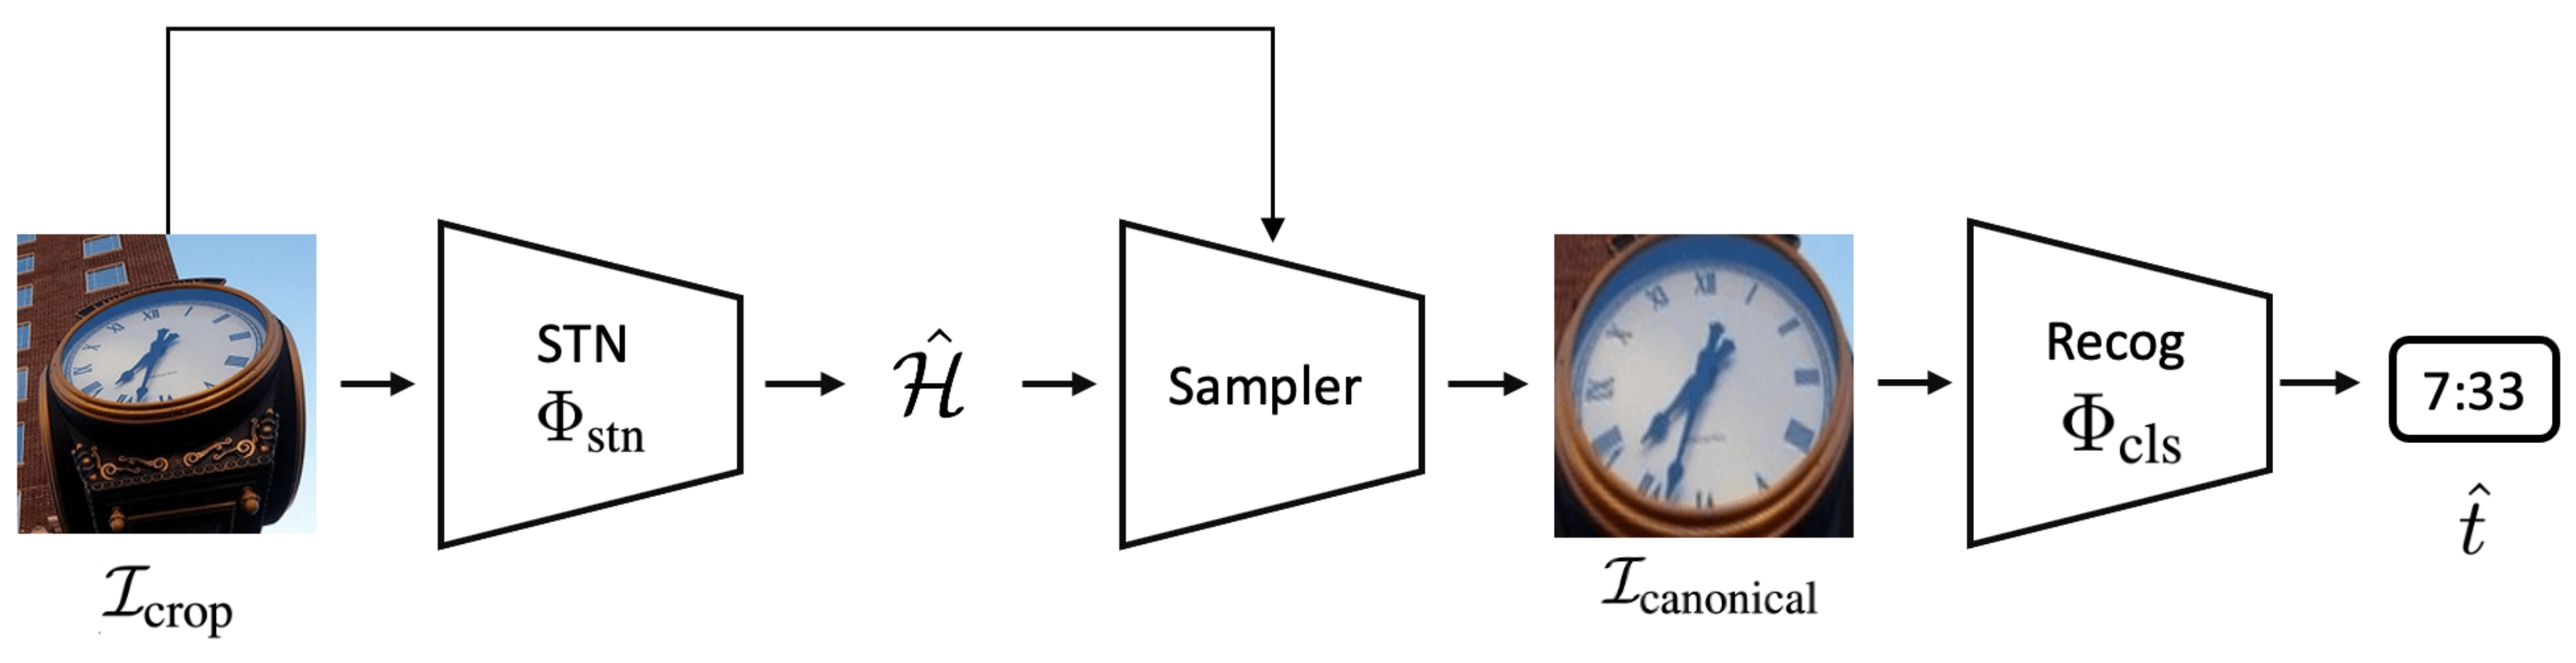
\includegraphics[width=0.9\textwidth]{figures/ArchitectureClock.png}
\caption{ClockDetector processing pipeline. Input frame undergoes YOLOv11 localisation, followed by spatial transformation network (STN) for perspective normalisation, and finally ResNet50 classification to predict time as one of 720 discrete minute classes~\cite{yang2024}.}
\label{fig:clock-pipeline}
\end{figure}

\textbf{Detection Stage}: The implementation uses YOLOv11n for initial clock detection. This lightweight model identifies clock faces within frames, providing bounding boxes for subsequent processing. The nano variant balances detection accuracy with processing speed, achieving sub-200ms inference even on CPU hardware. We use a confidence threshold of 0.25. Even though this high tolerance level might trigger more false positives, those are filtered out at later stages of the pipeline.

\textbf{Time Reading Methodology}: Yang et al.'s approach treats time reading as a classification problem rather than a regression. Their model divides the 12-hour clock face into 720 discrete classes, representing each minute as a unique entity. The architecture employs two key components:
\begin{itemize}
\item \textbf{Spatial Transformer Network (STN)}: Learns to normalise clock appearance by predicting homography parameters. This module transforms oblique views into frontal perspectives, standardising clock orientation regardless of camera angle.
\item \textbf{ResNet50 Classifier}: Processes the aligned clock image to predict one of 720 time classes. The classifier benefits from the STN's normalisation, focusing on time determination rather than handling perspective variations.
\end{itemize}

\begin{figure}[h]
\centering
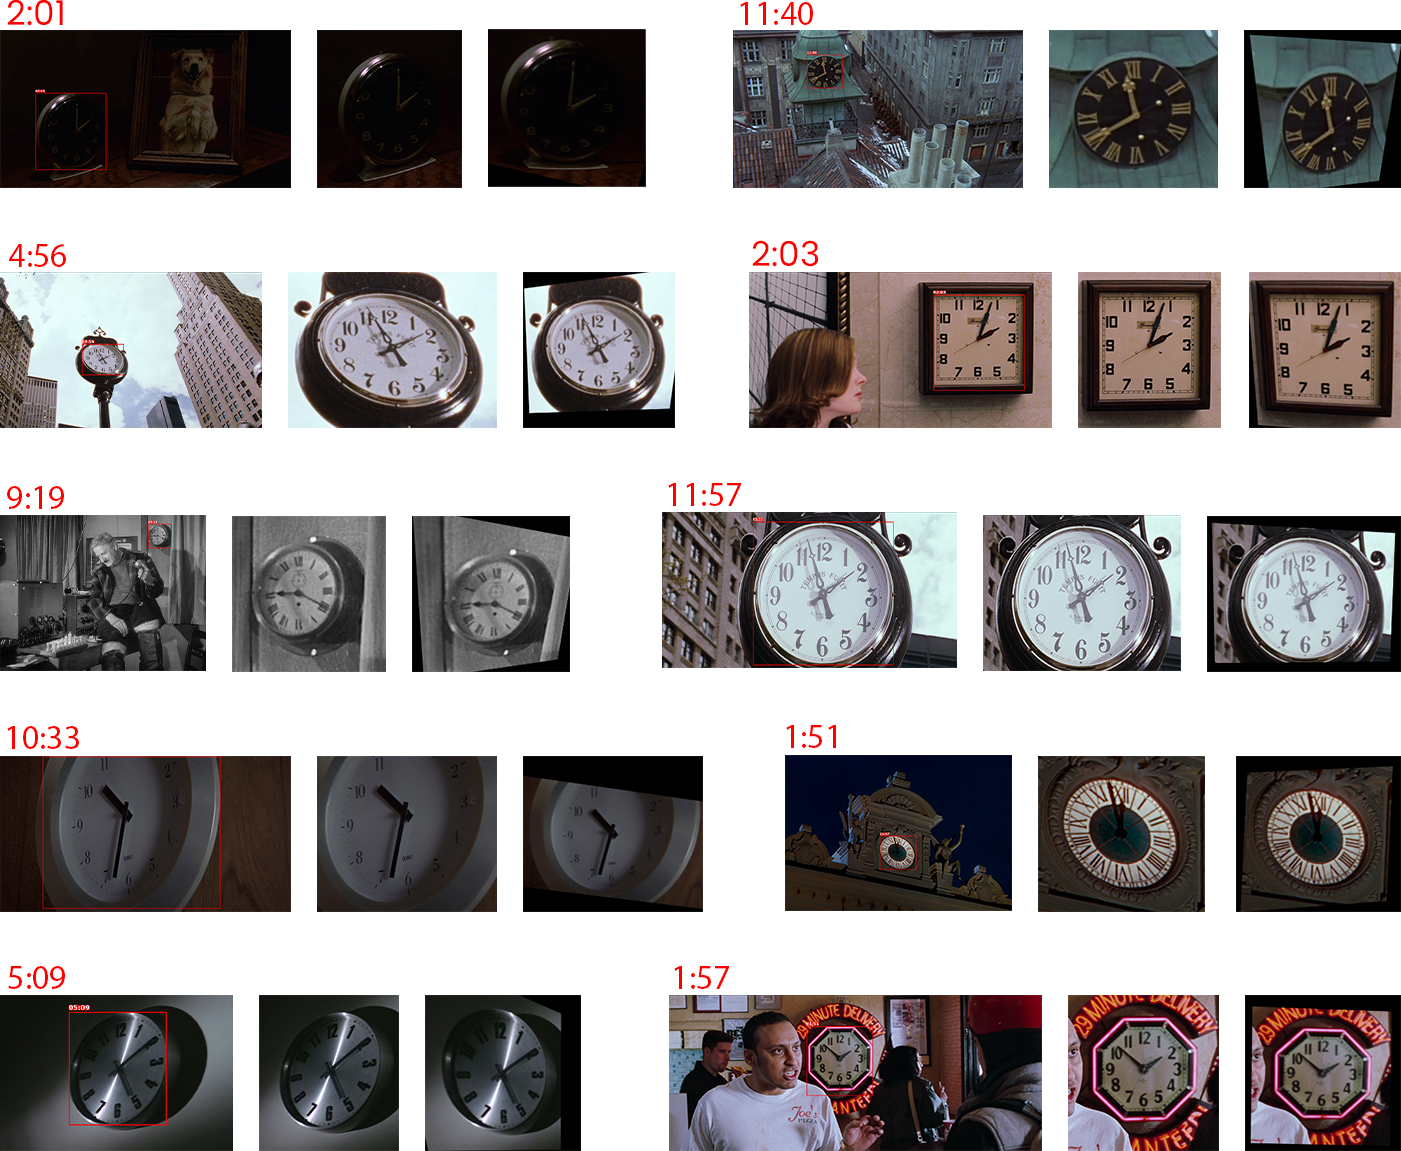
\includegraphics[width=0.9\textwidth]{figures/Clocks.png}
\caption{ClockDetector performance on challenging cases. Top row: Successful detections despite (a) partial occlusion, (b) extreme viewing angle, (c) motion blur. Bottom row: Failure cases due to (d) severe distortion, (e) ambiguous hand positions, (f) decorative clock design.}
\label{fig:clock-examples}
\end{figure}

Unlike the geometric analysis tested initially, this approach manages to accurately predict time even with some of the constraints: decorative or artistic clock faces with non-standard markers, partially occluded clock hands, variable hand designs (arrows, rectangles, ornate styles), shadows and reflections that confuse edge detection. The model's training on synthetic data with extensive augmentation enables generalisation to real-world clocks. Yang et al. report 80.4\% top-1 accuracy on COCO clock dataset.

\subsection{Digital Clocks}
Digital clock recognition presents a slightly different challenge than analog. Digital displays vary significantly in appearance from seven-segment LED displays to modern LCD screens. Each display type exhibits unique characteristics and varying contrast ratios.

\textbf{OCR Technologies}: Evaluation of available OCR solutions revealed significant performance differences for text detection. The seven-segment display study by Low et al. provides comprehensive analysis of OCR effectiveness on digital timepieces [24]. Their findings directly informed implementation choices for the detector.

Standard OCR tools like Tesseract and EasyOCR demonstrated poor performance on both regular text and seven-segment displays. Due to their limited training primarily on conventional fonts, they struggle to distinguish a high variety of digital clock faces. PaddleOCR, on the other hand, provided an optimal solution. Even though the study showed much higher scores of PARSeq's accuracy for seven-segment digits, PaddleOCR proved to be a good middle ground for performing text recognition of any kind.

\textbf{Processing Strategy}: Microwaves, smartphones, digital alarm clocks and watches, each presents time differently and in itself is a unique entity. Unfortunately, due to limitations of detection models like YOLO, attempting to localise the display and then perform OCR proved to be inaccurate. Missing simple alarm clock boxes or small seven-segment displays on other devices we had to opt for full OCR applied to the entire frame. This design trades computational efficiency for comprehensive coverage. The OCR engine examines all text-like regions, filtering results through time-pattern matching:

\begin{verbatim}
# Common time patterns (24-hour and 12-hour formats)
        self.time_patterns = [
            r'(\d{1,2}:\d{2}:\d{2})',                # Full time with seconds: 12:34:56
            r'(\d{1,2}:\d{2})',                      # Time without seconds: 12:34
            r'(\d{1,2}:\d{2}(?::\d{2})?\s*[APap][Mm])',  # 12-hour format: 12:34 PM
            r'(\d{1,2}[.:]\d{2}[.:]\d{2})',          # Alternative separators with seconds
            r'(\d{1,2}[.:]\d{2})',                   # Alternative separators without seconds
            r'(\d{1,2}\s*:\s*\d{2}\s*:\s*\d{2})',    # With spaces around colons
            r'(\d{1,2}\s*:\s*\d{2})',                # With spaces, no seconds
        ]
\end{verbatim}

\subsection{Validation and Error Reporting}
Reading individual timepieces is at the core of the detector, but we still need to add semantic value to the results and validate temporal continuity. The system maintains time progression records, comparing detected times from displays in either current or reference. 

For the sake of performance, if the script supervisor configures the detector for a specific time range, the detector would only request and process current frames instead of pairs. Since ground truth is now established through a given value, time detected in reference take is irrelevant. Otherwise, if no configuration for time range was provided, we utilise the first detected clock in the reference as ground truth for the scene's temporal validation. Clock detector identifies 3 main anomaly types:
\begin{itemize}
\item \textbf{Continuous flow}: Each subsequent clock after the first registered in the current frame should remain at a constant time or advance minimally.
\item \textbf{Time uniformity}: Every clock in a take should display near the same time.
\item \textbf{Narrative consistency}: The time of the scene should match across takes.
\end{itemize}

\section{DifferenceDetector}

\subsection{Detector Overview}
DifferenceDetector embodies a more conventional concept of automated continuity monitoring. It identifies visual changes between frame pairs that cannot be attributed to expected variations such as camera movement or actor motion. A similar idea was used in Pickup and Zisserman's 2009 study on film continuity where they computed pixel-wise differences between registered frames [5]. Unlike their pixel-based approach that flags every minor variation, this detector instead implements learned feature representations to distinguish meaningful changes from acceptable differences.

Traditional pixel-comparison would fail in production environment because it cannot differentiate between:
\begin{itemize}
\item A coffee mug that has genuinely moved (continuity error)
\item The same coffee mug appearing different due to lighting changes (acceptable variation)
\item A coffee mug at a slightly different angle due to camera movement (acceptable variation)
\end{itemize}

The detector was built upon the work completed by Sachdeva and Zisserman "The Change You Want to See" [22]. Their approach uses deep neural networks to extract high-level features from images at multiple spatial resolutions. These features capture object characteristics that remain consistent despite surface-level variations. When the model processes a coffee mug, it learns representations that are invariant to lighting changes and minor viewpoint shifts, enabling robust comparison between frames.

\subsection{Co-Attention Mechanism}
The architecture from Sachdeva and Zisserman employs co-attention mechanisms to establish implicit correspondences between frame pairs. This approach eliminates the need for explicit geometric registration, which often fails in real-world scenarios. Their architecture processes frame pairs through (see Figure 4.4):

\textbf{Feature Encoding}: A ResNet50 encoder extracts feature maps at three spatial resolutions from the last three blocks. These multi-scale representations capture both fine details and broader context.

\textbf{Co-Attention Module}: Each spatial location in one image's features attends to all locations in the other image's features. The attention mechanism computes:
\begin{itemize}
\item Query projections from the first image
\item Key projections from the second image
\item Attention weights through scaled dot-product
\item Weighted aggregation of features
\end{itemize}
The attended features are concatenated with the original features, providing both local information and cross-image context.

\textbf{Decoding}: A U-Net decoder with skip connections upsamples the conditioned features back to full resolution. Concurrent spatial and channel squeeze-and-excitation (scSE) blocks enhance feature representations.

\textbf{Detection}: A CenterNet head produces bounding box predictions for changed regions in both images simultaneously.

\begin{figure}[h]
\centering
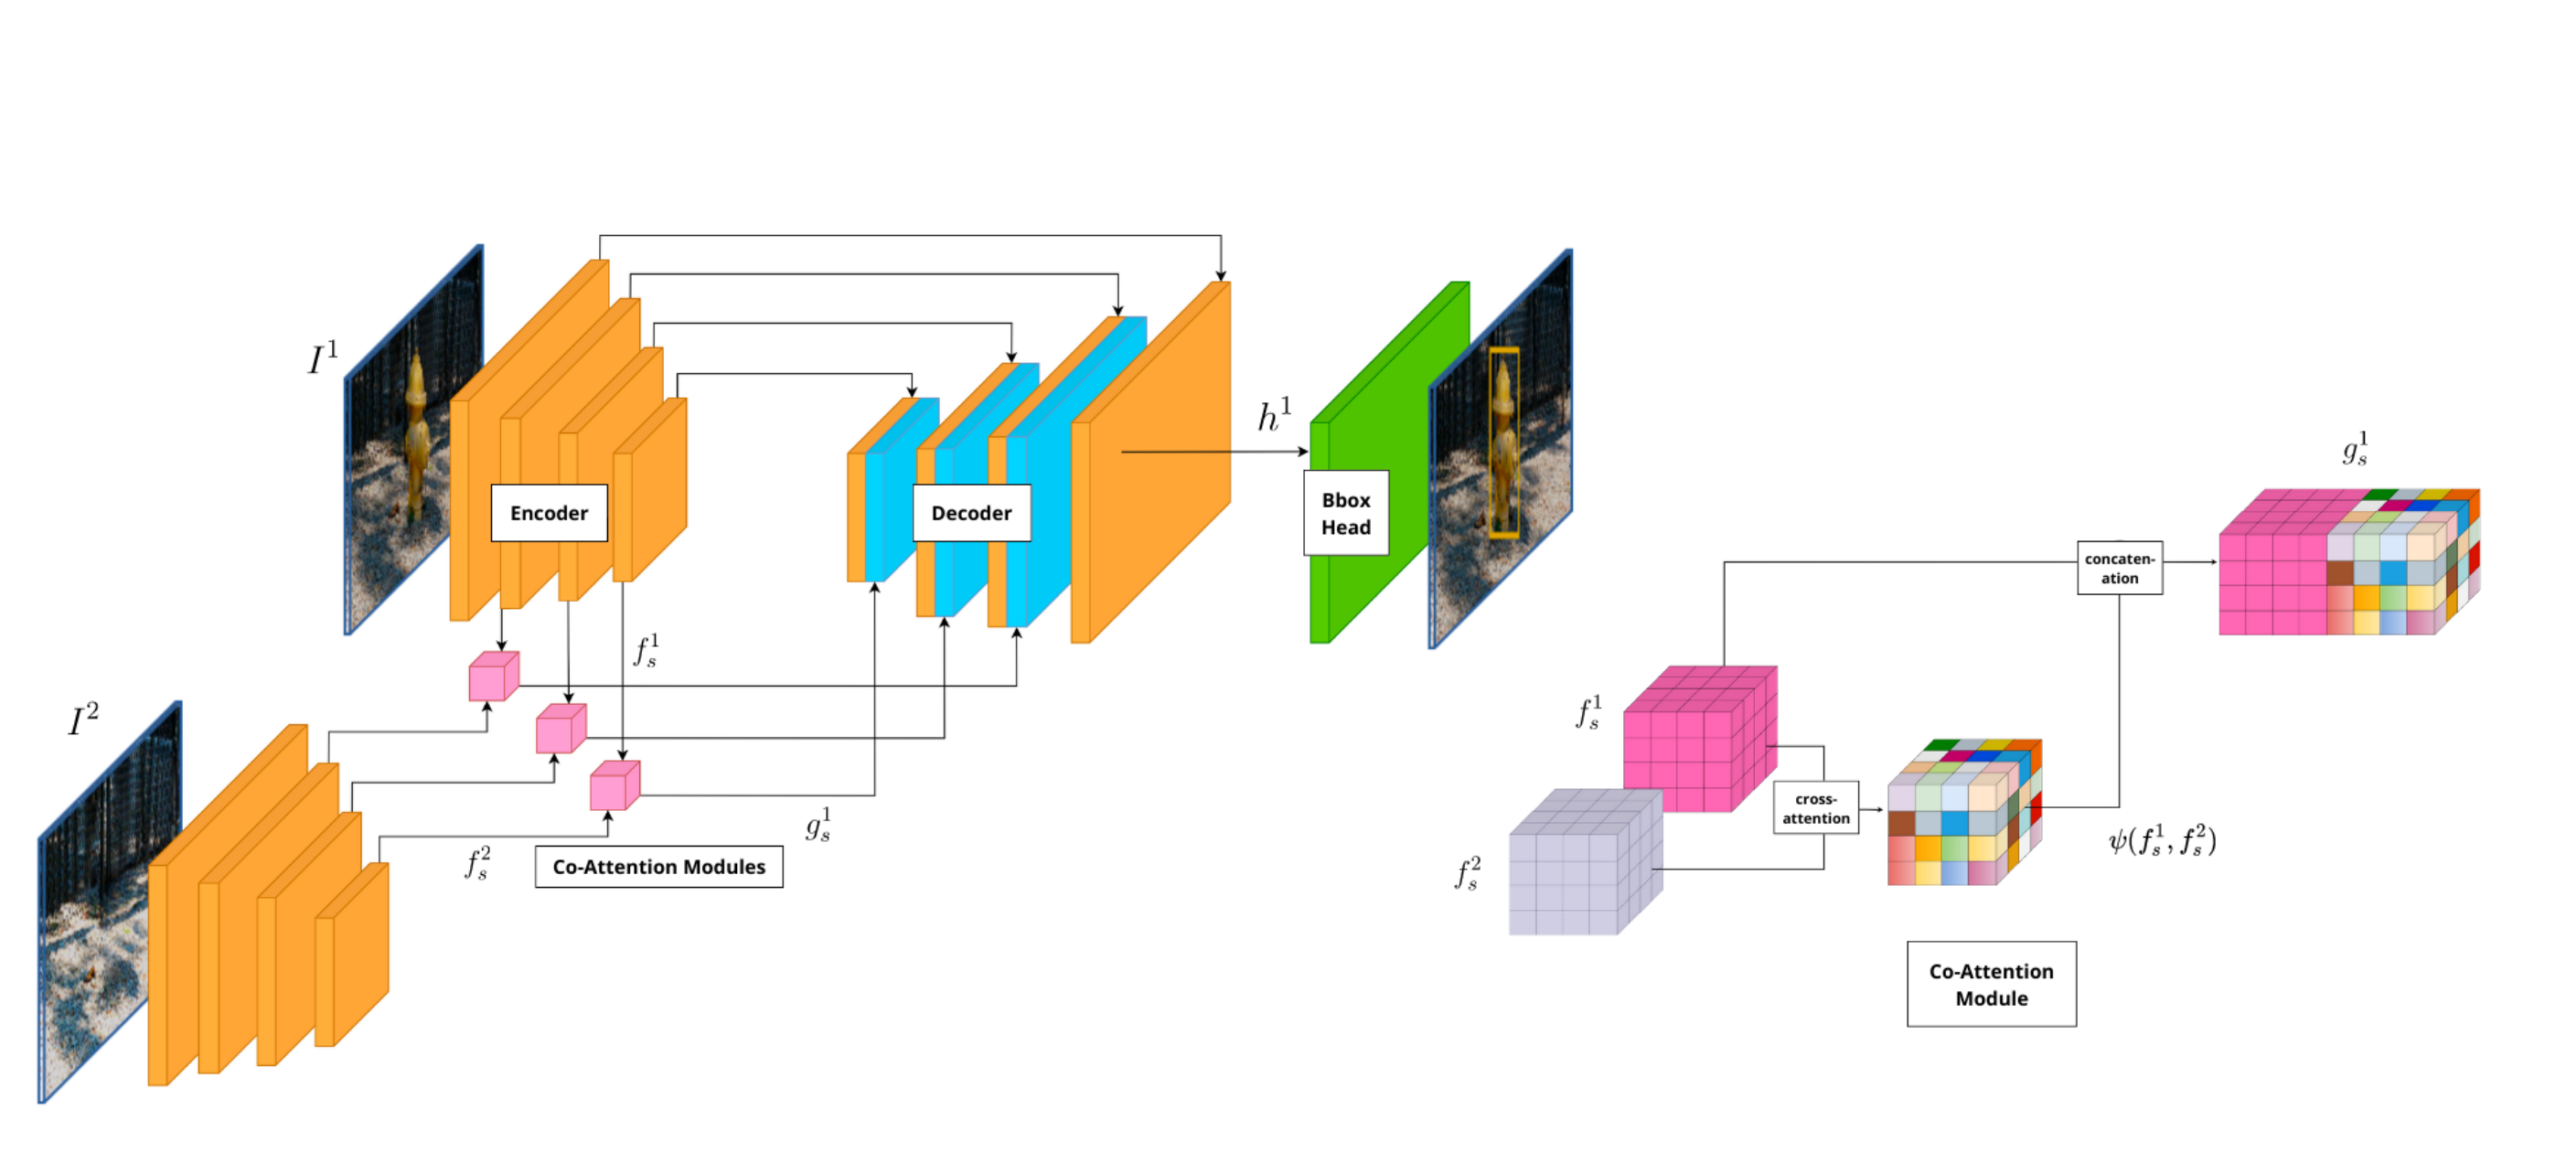
\includegraphics[width=0.9\textwidth]{figures/ArchitectureDifference.png}
\caption{DifferenceDetector architecture based on co-attention networks. ResNet50 extracts multi-scale features, co-attention modules establish implicit correspondences, and CenterNet heads detect changes without explicit registration~\cite{sachdeva2023change}.}
\label{fig:difference-architecture}
\end{figure}

\subsection{Specialised Masking and Filtering}
During principal photography, takes may slightly differentiate, especially when it comes to actors' performance interpretation. While Sachdeva and Zisserman's model excels at detecting changes between a pair of frames, it has no semantic context of narrative and filming variations.

Inspired by Pickup and Zisserman's observation about masking moving objects in their continuity error detection work [5], we implement a pre-processing stage that removes regions containing humans and animals before applying the change detection model. We use Detectron2's Mask R-CNN to identify humans and animals in both frames. These detected regions are expanded by 10\% to account for motion blur and edge uncertainties, then filled with neutral grey (128, 128, 128) to prevent artificial edges. This preprocessing ensures the change detection model focuses only on static scene elements where continuity errors can occur, rather than being distracted by unnecessary motion.

Neural network outputs undergo multi-stage filtering to produce practical results. Initial confidence filtering removes detections below 0.10. Subsequently, we filter by area (minimum 0.01\% of frame) and aspect ratio (0.1-10.0), eliminating sensor noise while preserving small significant changes. Finally, creature filtering suppresses detections with >30\% overlap with masked regions, accommodating partial occlusions while preventing false positives from motion.

\begin{figure}[h]
\centering
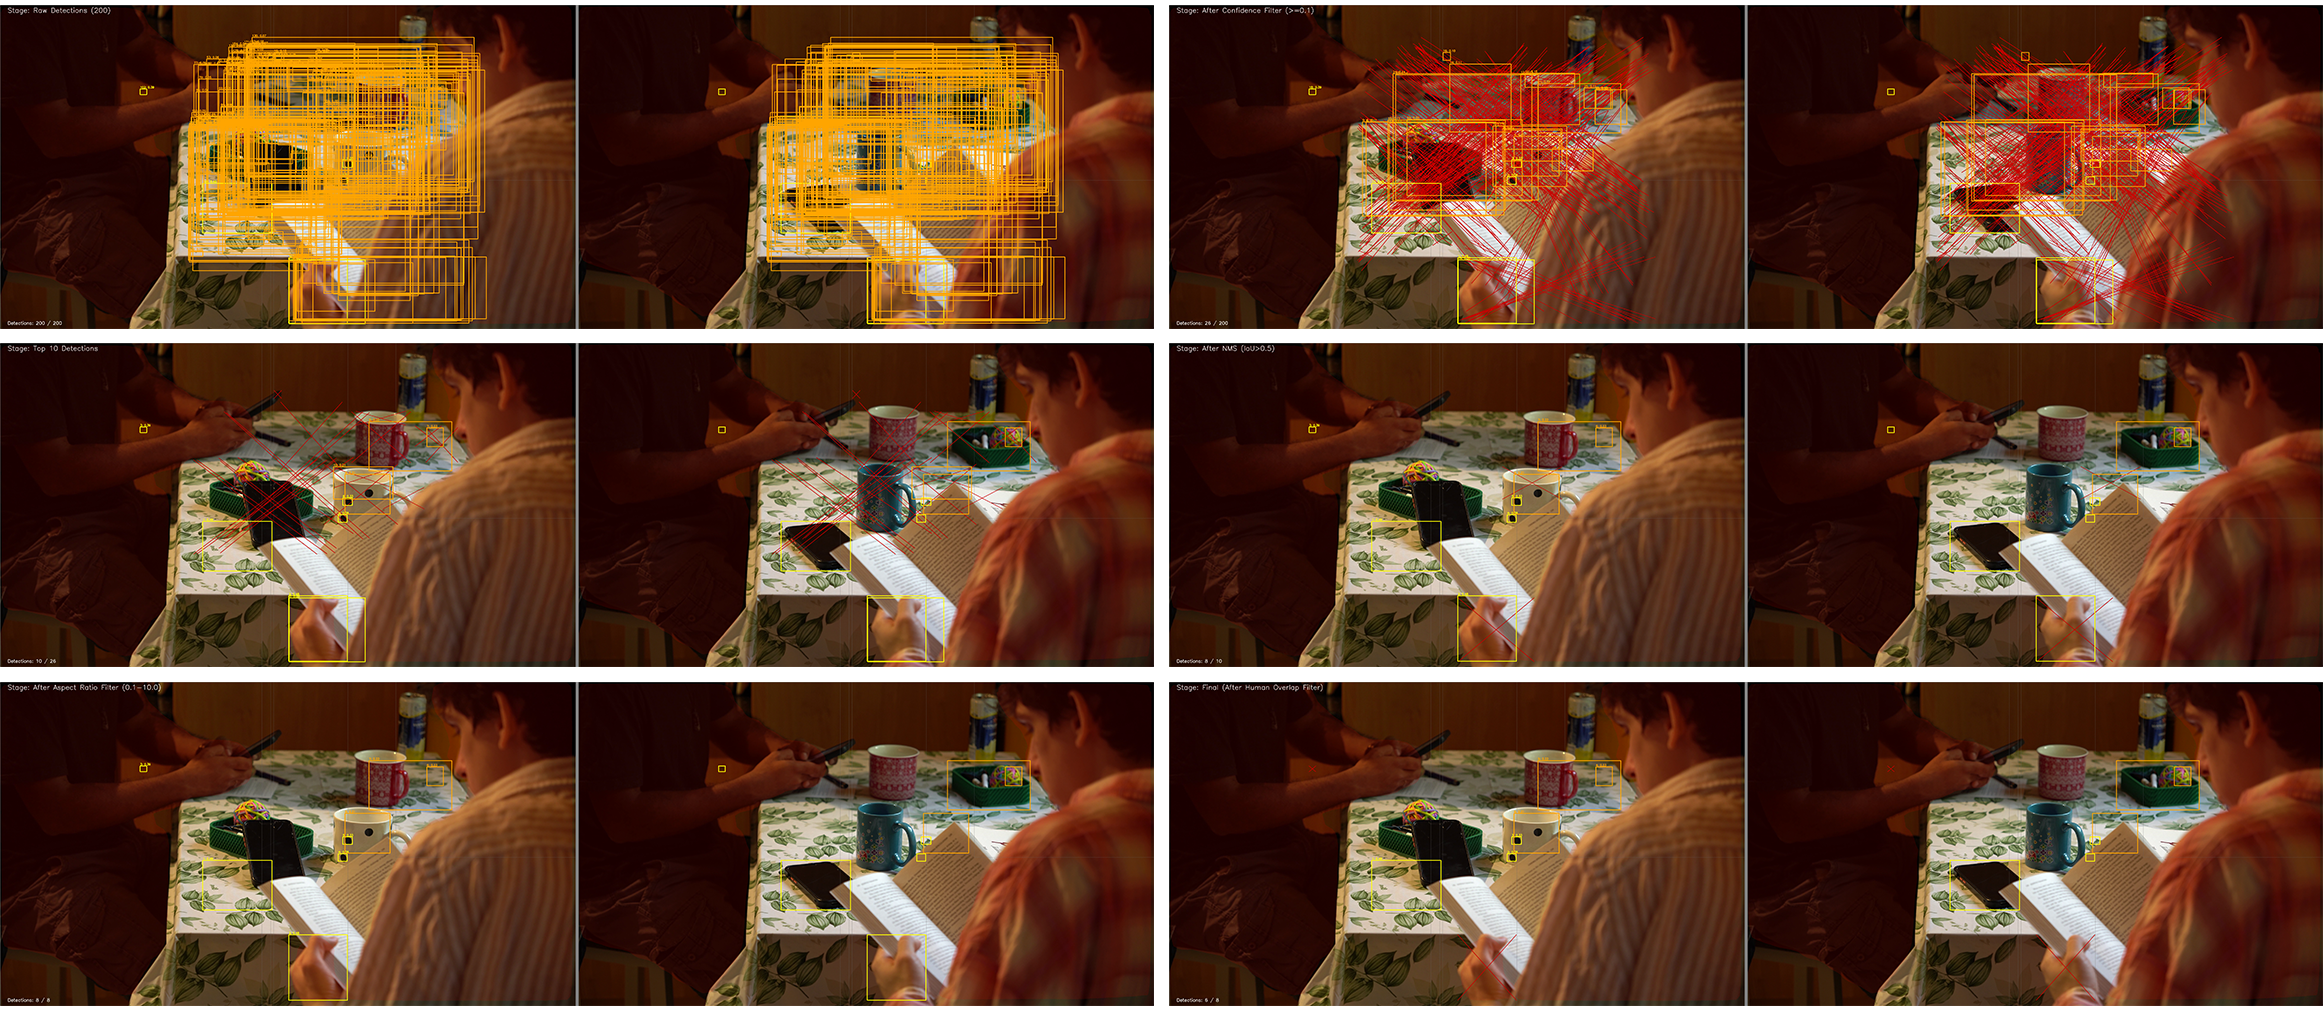
\includegraphics[width=0.9\textwidth]{figures/difference pipeline.png}
\caption{DifferenceDetector processing pipeline. (a) Reference and current frames. (b) Person segmentation masks (dilated for safety). (c) Co-attention difference map highlighting changes. (d) Final detections after filtering, showing moved prop (red box) while ignoring actor position changes.}
\label{fig:difference-pipeline}
\end{figure}

\subsection{Validation and Error Reporting}
Due to the already heavy computational complexity of the core implementation, we decided to opt for a streamlined error reporting approach. DifferenceDetector uses a unified "visual\_change" error type for all detections, avoiding the computational overhead of semantic classification to maintain real-time performance. Instead of categorising changes into types like "cup misplacement" or "missing remote", the system simply provides spatial data along with confidence scores. By focusing on accurate detection rather than interpretation, the detector delegates assessment to continuity professionals, where they can apply their expertise efficiently.

\section{Additional Features} 

\subsection{Parallel Processing}
Early prototyping showed that a universal detector would introduce enormous complexity and high performance overhead. Combining multiple technologies into one-for-all continuity monitoring process wouldn't be feasible. This constraint shaped the modular architecture, where specialised detectors operate in parallel to maintain real-time performance.

As previously discussed, each detector maintains its own PriorityQueueManager handling frame distribution. The framework spawns detector processes once a take is opened. It allows us to initialise detectors while the user prepares a new monitoring session. Once the capture starts we push frames to each detector's queue as they come. Non-blocking queues enable asynchronous processing: ClockDetector might analyse frame 10 whilst DifferenceDetector processes frame 7. Detection results are sent immediately back to the database and are rendered both as bounding boxes on the frame display and an alert in the detected anomalies table. Configurable queue limits prevent memory exhaustion without throttling faster detectors, ensuring consistent throughput regardless of individual detector complexity.

\subsection{Error Deduplication}
Production testing revealed that a single persistent error could generate hundreds of redundant alerts across multiple frames. The implementation employs two deduplication stages: real-time processing during capture and post-processing for batch analysis.

Real-time deduplication tracks errors across consecutive frames using spatial matching criteria. The system considers errors as matching when either their bounding boxes overlap by more than 50\%, IoU (Intersection over Union) > 0.5, or their centre points lie within 100 pixels of each other. Additionally, errors must originate from the same detector and contain matching description text. The algorithm requires errors to appear in consecutive frames to maintain continuity chains, marking them as inactive after a 5-frame absence. The database tracks continuous groups by storing first and last frame references. 

\subsection{Video Uploads}
During the development of the framework and detectors, assessment of the full workflow proved to have significant overhead: connecting capture devices, attempting to imitate specific anomalies and doing that repeatedly to mirror real production workflows. Implementing video upload proved to be a valuable addition to the rest of features to enhance both developers' and script supervisors' experiences. 

Upload uses OpenCV's \texttt{VideoCapture} to extract frames from video files at a configurable sample rate. The system loads the video file, calculates the sampling interval based on the scene's target frame rate versus the video's native frame rate, then iterates through frames saving them as individual PNG files with lossless compression (level 3) via the storage service, which is consistent with the live capture. With \texttt{BatchProcessor} videos are handled in parallel segments using Python's \texttt{ThreadPoolExecutor} to increase upload speed.
\chapter{Evaluation}

\section{Evaluation Methodology}
Evaluating a real-time continuity monitoring system requires balancing traditional computer vision metrics with production-specific constraints. Unlike conventional object detection benchmarks that prioritise accuracy alone, film production demands both precision and speed. This evaluation therefore examines three main properties: detection accuracy to ensure reliability, processing speed to enable real-time operation and practical applicability within production workflows.

\subsection{Evaluation Metrics}
\textbf{mAP (mean Average Precision)}: Following standard object detection evaluation practices, we adopt mAP as our primary accuracy metric for DifferenceDetector. Modern detection systems including YOLOv11 [16] and Detectron2 [18] utilise mAP at various IoU thresholds to comprehensively assess detection quality.

\textbf{Accuracy}: ClockDetector in its nature solves classification problem, so even though it utilises YOLOv11 for object detection, the overall performance can be summarised using accuracy, precision, recall and F1.

\textbf{Time to Detection (TtD)}: End-to-end processing time from frame capture to result, ensuring detection completes within production reset windows.

\textbf{False Positive/Negative Rates}: Separate error analysis since missed continuity errors cost significantly more than false alerts in post-production.

\subsection{Test Environment}
We deliberately chose consumer-grade hardware for evaluation to reflect realistic deployment scenarios:
\begin{itemize}
\item CPU: Intel Core i9-11900 (8 cores, 5.3GHz boost)
\item GPU: NVIDIA RTX 3050 (4GB VRAM, GPU acceleration enabled)
\item RAM: 32GB DDR4-3200
\item Storage: 1TB NVMe SSD
\item Total cost: approximately £2,000
\end{itemize}

\subsection{Dataset Composition}
The selection of evaluation datasets presented unique challenges, as no existing benchmarks specifically address film continuity detection. To properly evaluate the overall performance we use tailored datasets for each detector. Table 5.1 summarises the dataset characteristics and their evaluation purposes.

\begin{table}[h]
\centering
\caption{Dataset Composition for both ClockDetector and DifferenceDetector}
\label{tab:datasets}
\begin{tabular}{llll}
\toprule
\textbf{Dataset} & \textbf{Type} & \textbf{Size} & \textbf{Purpose} \\
\midrule
\multicolumn{4}{l}{\textit{ClockDetector Datasets}} \\
ClockMovies & Real film footage & 1,131 images & Analogue clock variety \\
Synthetic digital & Generated & 100 images & Digital clock precision \\
\midrule
\multicolumn{4}{l}{\textit{DifferenceDetector Datasets}} \\
COCO-Inpainted (small) & Modified photos & 1,655 pairs & Small object changes (<32² px) \\
COCO-Inpainted (medium) & Modified photos & 1,747 pairs & Medium objects (32²-96² px) \\
COCO-Inpainted (large) & Modified photos & 1,006 pairs & Large objects (>96² px) \\
SynthText-Change & Synthetic & 5,000 pairs & Text modifications \\
VIRAT-STD & Surveillance & 26,155 pairs & Outdoor scenes \\
Kubric-Change & 3D rendered & 1,604 pairs & Geometric transformations \\
\bottomrule
\end{tabular}
\end{table}

\section{Performance Analysis}

\subsection{ClockDetector}
ClockDetector demonstrated robust classification performance across 1,231 test images from film footage and synthetic clocks. The detector overall achieved:
\begin{itemize}
\item Accuracy: 75.0\% (923/1231 correct classifications)
\item Precision: 81.4\% (923/1134 true positives among detections)
\item Recall: 75.0\% (923/1231 clocks correctly identified and read)
\item F1 Score: 0.78
\end{itemize}

These metrics reveal balanced performance between precision and recall, with the system correctly reading time in 81.4\% of detected clocks whilst identifying 75\% of all clocks in the dataset. Digital and analog clocks showed distinct performance characteristics (Table 5.2):

\begin{table}[h]
\centering
\caption{ClockDetector Performance for each clock type}
\label{tab:clock-performance}
\begin{tabular}{llllll}
\toprule
\textbf{Clock Type} & \textbf{Total} & \textbf{Correct} & \textbf{Accuracy} & \textbf{Precision} & \textbf{Recall} \\
\midrule
Analog & 1,131 & 832 & 73.6\% & 80.3\% & 89.8\% \\
Digital & 100 & 91 & 91.0\% & 92.9\% & 97.8\% \\
\bottomrule
\end{tabular}
\end{table}

Digital clock recognition performed well at a high 91\% accuracy through PaddleOCR's text detection capabilities. However, the limited test set of 100 images indicates a need for more thorough evaluation on larger datasets to validate this performance across diverse digital display types and more complex scene setups.

Analog clocks proved more challenging at 73.6\% accuracy. While this falls below Yang et al.'s reported ~80\% [23], our precision of 80.3\% aligns more closely with their findings. This discrepancy likely stems from our addition of YOLOv11 as a detection layer before time reading, which introduces an extra failure point where clocks might not be detected at all, thus reducing overall accuracy whilst maintaining high precision on detected clocks. The systematic challenges for analog clock recognition included:
\begin{itemize}
\item Extreme viewing angles where STN homography failed to normalise the clock face
\item Decorative faces lacking clear hour markers, common in period films
\item Low-contrast scenes typical in film noir where clock hands blend with backgrounds
\end{itemize}

Time to Detection averaged 1.92 seconds per frame pair, with the majority of processing time (83.1\%) consumed by the time reading. Either the STN and ResNet50 pipeline for analog clocks or PaddleOCR scanning for digital displays. 

The error distribution reveals that most errors occurred during time reading rather than detection. YOLOv11 successfully identifies clocks in 92.1\% of images. 
\begin{itemize}
\item False Negatives (No detection): 97 images where no clock was found
\item False Positives (Incorrect reading): 211 images where clocks were detected but time was misread
\end{itemize}

As previously discussed we aim for low miss rates (false negatives), since it leads to costly post production fixes. Evaluation revealed that ClockDetector outperforms in this metric with just 7.9\% failures.

\subsection{DifferenceDetector}
DifferenceDetector achieved 60.7\% mean Average Precision (mAP) at IoU 0.5 across 38,167 test frame pairs, almost matching the baseline performance reported by Sachdeva and Zisserman [22]. This demonstrates successful adaptation of their co-attention architecture to film production contexts, despite our additional masking and filtering stages. We can see detector's strength and limitations from its performance on different datasets (Table 5.3):

\begin{table}[h]
\centering
\caption{DifferenceDetector performance across evaluation datasets}
\label{tab:difference-performance}
\begin{tabular}{llll}
\toprule
\textbf{Dataset} & \textbf{mAP} & \textbf{Key Characteristics} & \textbf{Frames} \\
\midrule
COCO small & 0.462 & Challenging small objects & 1,655 \\
COCO medium & 0.787 & Optimal detection range & 1,747 \\
COCO large & 0.850 & Easiest size category & 1,006 \\
COCO combined & 0.627 & - & 4,408 \\
SynthText-Change & 0.890 & High contrast text & 5,000 \\
VIRAT-STD & 0.540 & Outdoor lighting variations & 26,155 \\
Kubric-Change & 0.761 & 3D transformations & 1,604 \\
\bottomrule
\end{tabular}
\end{table}

Performance correlates strongly with object size, dropping from 85\% for large changes to 46.2\% for small objects. Outdoor surveillance footage with dynamic lighting conditions poses significant challenges for the detector, along with other kinds of occlusions and fine detail. The consistent performance across synthetic and real-world datasets suggests reasonable generalisation to production footage.

Time to Detection averaged 6.37 seconds per frame pair, substantially longer than ClockDetector. This processing time reflects the computational complexity of co-attention mechanisms operating at multiple feature scales.

\subsection{Detection Accuracy}
The evaluation results reveal a critical distinction between achieving technical benchmarks and production viability. In Section 3.1.2, we established human script supervisor accuracy at 75-80\% over 10-14 hour production days, based on vigilance task research [9]. Against this baseline, ClockDetector's 75\% accuracy technically meets human performance levels, suggesting reliable deployment potential for temporal continuity monitoring.

However, DifferenceDetector's 60.7\% mAP falls substantially short of human capability. This 15-20\% performance gap becomes more pronounced considering the detector's sensitivity to environmental conditions. Outdoor scenes achieved only 54\% mAP versus 89\% on high-contrast synthetic data. Such variance indicates unreliable performance across diverse production environments, from controlled studio sets to dynamic location shoots.

These results definitively position CAM-F as an assistive rather than autonomous system. ClockDetector can reliably flag temporal inconsistencies for supervisor verification, while DifferenceDetector serves best as a preliminary filter for obvious spatial changes.

\subsection{Real-time Viability}
Determining real-time performance requires more nuance than simple frame rates. We developed a custom metric that calculates the maximum capture frame rate sustainable within production constraints, accounting for processing backlogs during takes and recovery during reset windows. We introduce a Production-Aligned Frame Rate (PAFR) metric that calculates the maximum capture rate sustainable during filming whilst guaranteeing all processing completes before the next take begins.

Given:
\begin{itemize}
\item x = time-to-detect per frame pair (seconds)
\item y = capture frame rate (fps)
\item S = typical take duration (seconds)
\item R = reset window between takes (seconds)
\end{itemize}

The system operates in one of two modes:

\textbf{Strict real-time}: Processing keeps pace with capture, requiring:
$$y \leq \frac{1}{x}$$

\textbf{Production real-time}: Frames queue during filming but clear during reset. The queue grows at $(y - \frac{1}{x})$ fps during the S-second take, creating a backlog:
$$q(S) = \left(y - \frac{1}{x}\right) \cdot S$$

These frames require time to process:
$$T_{\text{clear}} = S \cdot (y \cdot x - 1)$$

To finish before the next take, we need $T_{\text{clear}} \leq R$, yielding maximum sustainable frame rate:
$$y_{\text{max}} = \frac{\frac{R}{S} + 1}{x}$$

As we previously discussed in the system requirements, workflows and timings differ significantly depending on the size of the production. For the sake of grounding the system and evaluating its temporal performance we assume the most common scenario, where each take is about 45 seconds, while reset time is 5 minutes. In such case:

\textbf{ClockDetector Analysis}

With x = 1.92s per frame pair:
\begin{itemize}
\item Strict real-time: $y \leq \frac{1}{1.92} = 0.52$ fps
\item Production real-time (45s take, 300s reset):
$$y_{\text{max}} = \frac{\frac{300}{45} + 1}{1.92} = \frac{7.67}{1.92} = 4.0 \text{ fps}$$
\end{itemize}

With the PAFR of 4fps, ClockDetector would capture every 6th frame of the 24fps incoming feed.

\textbf{DifferenceDetector Analysis}

With x = 6.37s per frame pair:
\begin{itemize}
\item Strict real-time: $y \leq \frac{1}{6.37} = 0.16$ fps
\item Production real-time (45s take, 300s reset):
$$y_{\text{max}} = \frac{\frac{300}{45} + 1}{6.37} = \frac{7.67}{6.37} = 1.2 \text{ fps}$$
\end{itemize}

With the PAFR of 1.2fps, DifferenceDetector would capture approximately every 20th frame of the 24fps incoming feed.

\begin{figure}[h]
\centering
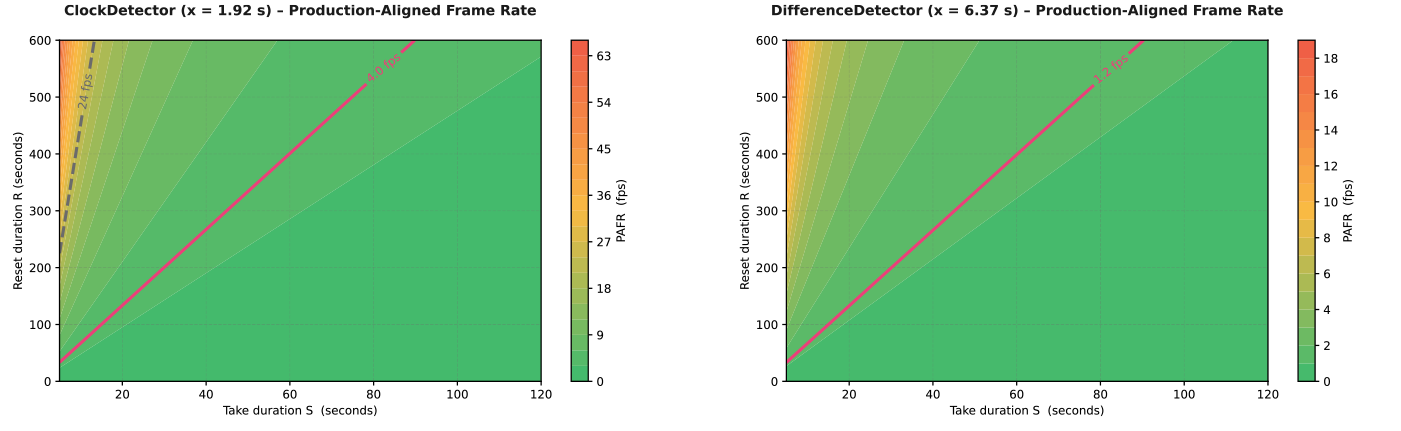
\includegraphics[width=\textwidth]{figures/PAFRplot.png}
\caption{Production-Aligned Frame Rate (PAFR) analysis showing the relationship between capture frame rate and backlog clearing time for both detectors. The intersection of each detector curve with the 300-second reset window (red dashed line) determines maximum sustainable frame rates: 4.0 fps for ClockDetector and 1.2 fps for DifferenceDetector. The shaded region indicates frame rates that would cause production delays by exceeding available reset time. System-wide performance is constrained by the slowest detector at 1.2 fps.}
\label{fig:pafr}
\end{figure}

When running multiple detectors concurrently, the system must synchronise frame distribution to maintain consistency. The slowest detector constrains the entire pipeline to 1.2fps in our case. This infrequent sampling proves sufficient as continuity errors typically persist for some time. The PAFR metric aims to confine CAM-F within its limitations and ensure that processing backlogs never exceed reset windows, guaranteeing detection results arrive before the next take begins without production delays. Figure 5.1 visualises these PAFR calculations across different production scenarios.

\subsection{Workflow Integration Testing}
Integration testing evaluated CAM-F under simulated production conditions using staged scenes with 12 planted continuity errors. Testing consisted of static takes from multiple angles and motion sequences with both actor and camera movement. Each scene employed carefully tuned detector configurations, which are available in the UI, demonstrating the importance of scene-specific parameter adjustment for optimal performance.

\textbf{Test Configuration and Results}

The system processed approximately 30 seconds of footage at 1 FPS capture rate, completing detection within 3 minutes post-take. This performance aligns with our PAFR metric calculations, which allows up to 1.1 FPS for this take-reset configuration to maintain production workflow compatibility. The interface successfully displayed real-time detection results and we managed to generate structured reports without any disruptions.

CAM-F detected 10 out of 12 planted errors (83.3\% recall) with 71-77\% precision. Static scenes detected 7/9 errors (77.8\%) with 3-4 false positives (see Figures 5.2 and 4.5), while motion scenes achieved perfect detection (3/3) with zero false positives (see Figure 5.3). This performance exceeds the dataset evaluation results, where DifferenceDetector achieved only 60.7\% mAP. The improved accuracy partly comes from the limited test cases, but more significantly from the fundamental difference in image quality. Benchmark datasets contain images of highly variable quality: compressed web images, surveillance footage and amateur photography. Professional film production maintains consistent high resolution and visual clarity. Modern cameras can capture at 4K or even higher with proper lighting and focus. This quality consistency gives detection algorithms cleaner features to analyse and improves object detection. Our results suggest that CAM-F may perform more reliably in actual production environments than synthetic benchmarks predict, as professional footage provides optimal conditions for computer vision algorithms.

\begin{figure}[h]
\centering
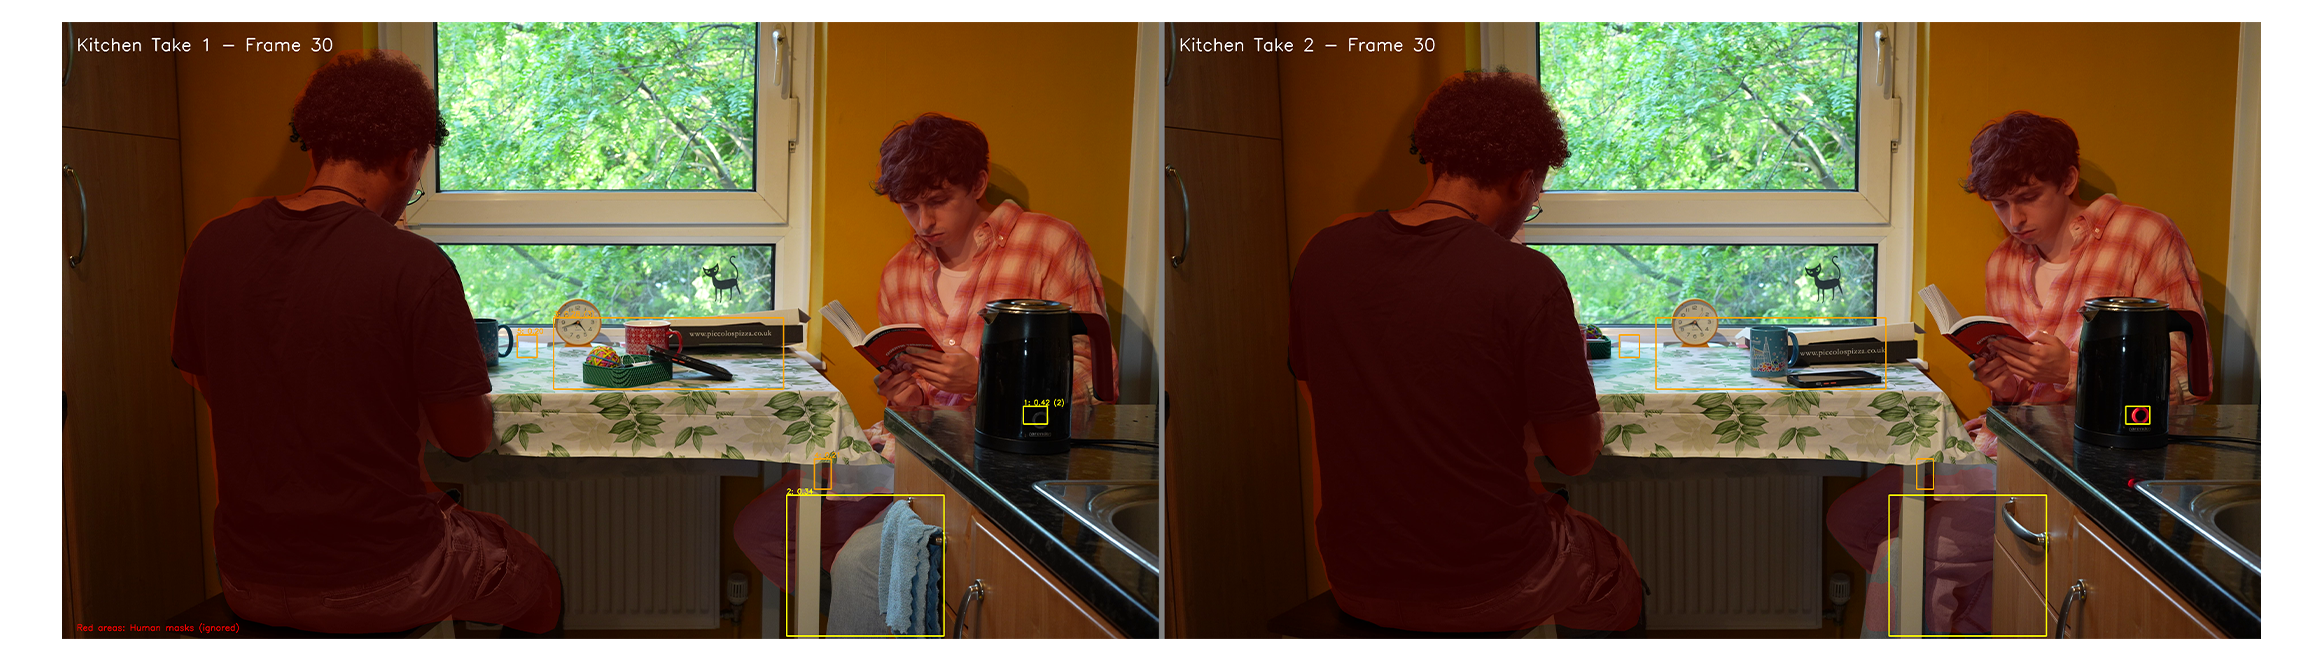
\includegraphics[width=\textwidth]{figures/statictest.png}
\caption{Integration test results from static scene. Wide-angle shot captured over 30 seconds at 1 fps, showing frame 30 with detection overlay.}
\label{fig:static-shots}
\end{figure}

The motion scene's perfect detection rate requires important clarification. We achieved 3/3 error detection using 2 FPS capture over 15 seconds (see Figure 5.3), which would exceed acceptable PAFR. Initial testing at the standard 1 FPS rate missed one of the errors. A book at the frame edge during camera movement appeared only briefly between sampled frames. The error became detectable only when we doubled the capture rate to 2 FPS. This shows a fundamental limitation of PAFR-constrained processing. Motion-heavy takes are much more likely to have temporal windows where errors exist for mere fractions of a second. At 1 FPS, the system samples every 24th frame, creating about 0.96-second blind spots where such errors escape detection entirely. CAM-F's effectiveness, in its current computational capabilities, diminishes proportionally with scene's dynamics, making it most suitable for dialogue scenes and static setups rather than action sequences.

\begin{figure}[h]
\centering
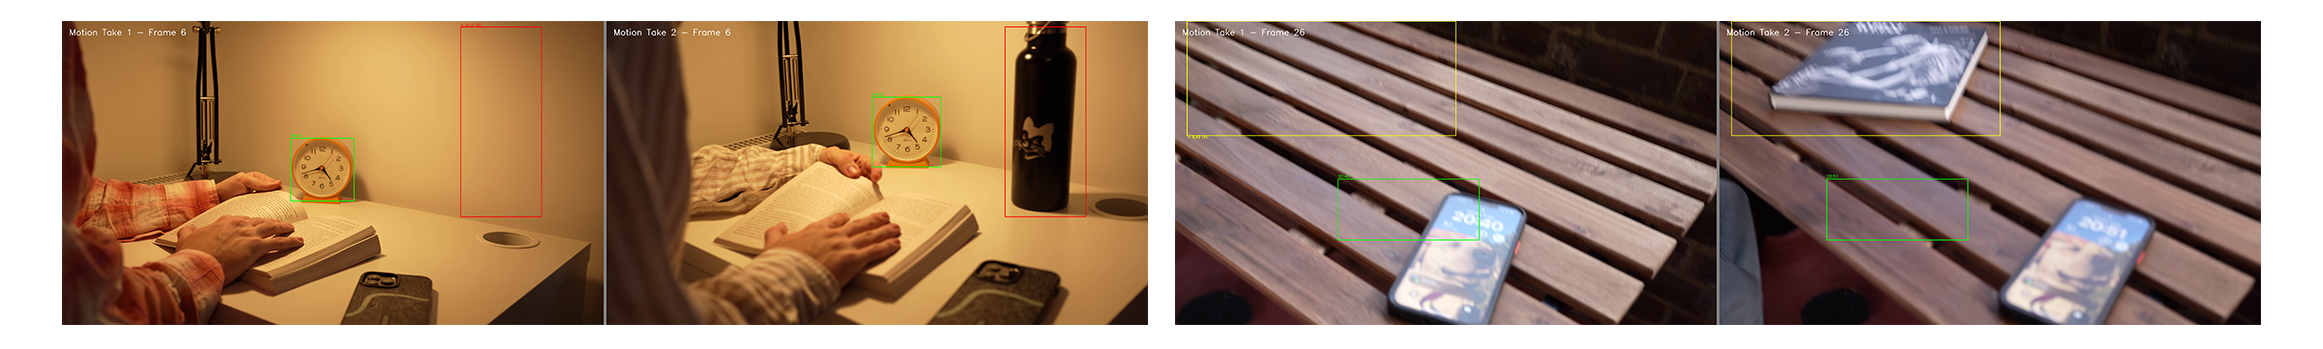
\includegraphics[width=\textwidth]{figures/motiontest.png}
\caption{Integration test results from dynamic scene with camera movement. 15-second sequence captured at 2 fps, showing frames 6 and 26. Detection performance remained consistent despite motion, though higher capture rate was required to detect transient errors.}
\label{fig:dynamic-shots}
\end{figure}

The UI effectively supported the complete workflow from capture to documentation. Detection results appeared immediately in the error log with clear frame references and confidence scores. The false positive flagging interface allowed us to mark those incorrect detections we got in the experiment, removing them from the active error list. The PDF export contains all the findings and we could also add extra notes for clarity. This end-to-end workflow successfully imitated actual production practices where script supervisors quickly verify, annotate, and distribute continuity information. The system's ability to generate structured documentation within minutes of take completion shows us potential in its practical readiness for set deployment.

\begin{figure}[h]
\centering
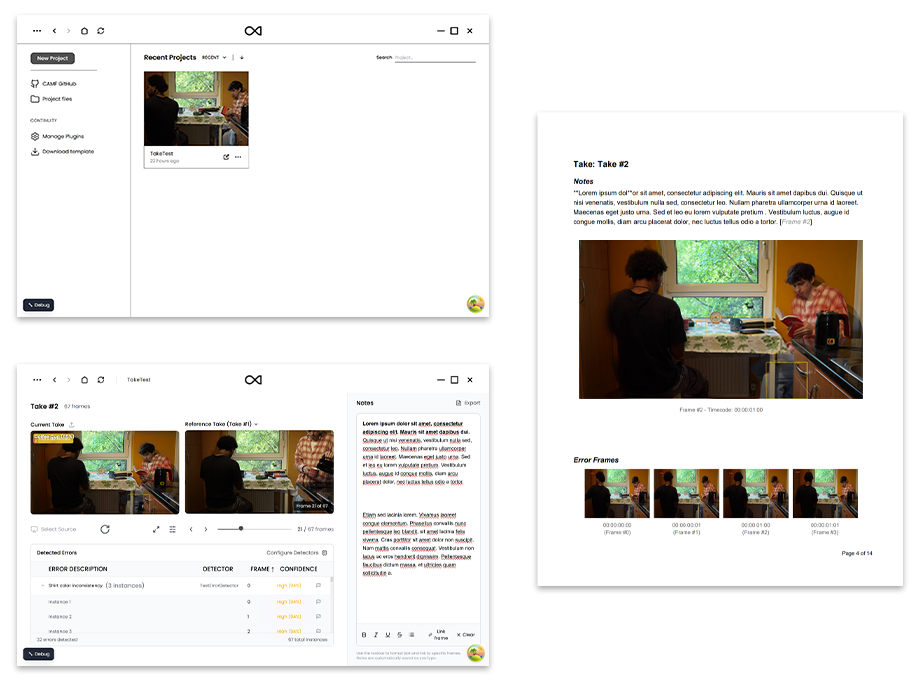
\includegraphics[width=\textwidth]{figures/app.png}
\caption{CAM-F workflow interface showing real-time monitoring dashboard, detection results and generated PDF continuity report.}
\label{fig:app-interface}
\end{figure}

\section{Discussion}

\subsection{Results Overview}
The evaluation demonstrates that CAM-F achieves partial fulfilment of its design objectives. The system successfully implements real-time continuity monitoring within production constraints, processing all captured frames before subsequent takes commence. However, performance metrics reveal significant variance between detector implementations, with ClockDetector achieving human-equivalent accuracy and DifferenceDetector operating substantially below production needs, though integration testing revealed more promising results.

ClockDetector's 75\% accuracy aligns with the human performance baseline of 75-80\%, that we established based on study by Warm et al. [9] for sustained vigilance tasks, suggesting viable deployment potential for temporal continuity monitoring. The detector's 80.3\% precision on detected analog clocks demonstrates reliable performance when objects are successfully identified. Digital clock recognition also performed exceptionally well at 91\% accuracy through PaddleOCR, though it can be explained with a limited test set.

DifferenceDetector's 60.7\% mAP falls 15-20\% below human capability, rendering it suitable only as a preliminary filter rather than autonomous detection. Performance variance across datasets, from 89\% on high-contrast synthetic data to 54\% on outdoor surveillance footage, indicates environmental sensitivity that might be problematic across diverse production settings. However, integration testing production-quality footage achieved 83.3\% overall recall, suggesting that real environments on-set with consistent high-resolution capture may yield substantially better performance than synthetic benchmarks indicate. Nevertheless, the detector successfully adapts Sachdeva and Zisserman's co-attention architecture [22] to production contexts, demonstrating feasibility even if practical limitations remain.

The Production-Aligned Frame Rate metric reveals system-wide performance constrained to 1.2fps by DifferenceDetector's 6.37-second processing time. Whilst this appears restrictive compared to standard 24fps capture, Schmidt et al. [25] demonstrated that sampling films at one frame per second provides sufficient temporal resolution for narrative analysis, as consecutive frames share approximately 90\% similarity.

\subsection{Limitation Analysis}
\textbf{Error Coverage}: The current implementation partially addresses only two of the four major continuity error categories identified in Table 2.1. ClockDetector monitors temporal continuity through time-display analysis, while DifferenceDetector identifies spatial continuity violations through object displacement. However, action continuity and technical continuity remain entirely unaddressed. Combined, proposed detectors handle about 15\% of various continuity anomalies.

\textbf{FPS Constraints}: The 1.2 fps sampling rate, constrained by DifferenceDetector's processing time, introduces temporal blind spots in continuity monitoring. At this rate, the system captures approximately every 20th frame from standard 24fps footage, creating 0.79-second gaps between analysed frames. Critical limitations emerge in high-motion scenarios where camera movement or rapid set changes could cause errors to appear and disappear between sampled frames.

\textbf{Frame Alignment}: The absence of temporal synchronisation between reference and current takes creates systematic comparison errors. Takes rarely begin at precisely the same narrative moment due to the manual nature of capture controls. Spacial alignment is another issue that may arise through accidental camera adjustments or specific creative decisions. Since both implemented detectors are agnostic to temporal and spatial misalignment we prioritised other features over this one. However, in a reliable system with high monitoring standards, it is an essential preprocessing step.

\textbf{Dataset Validity}: The evaluation relies entirely on synthetic and modified datasets rather than authentic film footage. Since none of it is available in public access, we're left to use detector specific compositions. COCO-Inpainted image and other datasets we used lack the visual and functional characteristics of real film production.
% Write your conclusions here
\label{Conclusions} % If you need a label for this chapter

% Example text



All good projects conclude with an objective evaluation of the project's successes and failures and suggestions for future work which can take the project further. It is important to understand that there is no such thing as a perfect project. 

Even the very best pieces of work have their limitations and you are expected to provide a proper critical appraisal of what you have done. Your assessors are bound to spot the limitations of your work and you are expected to be able to do the same.


% Back matter
\backmatter

% Bibliography
% Bibliography using BibLaTeX
\printbibliography[heading=bibintoc,title={References}]

% Declarations (NEW requirement from 2024-25)
% Must be positioned after References and before Appendices
% Declarations Chapter
% Required from 2024-25 academic year onwards
% This chapter should be positioned after References and before Appendices
\chapter*{Declarations}
\addcontentsline{toc}{chapter}{Declarations}

\section*{Declaration of Originality}

I hereby declare that the work presented in this thesis is my own unless otherwise stated. To the best of my knowledge the work is original and ideas developed in collaboration with others have been appropriately referenced.

\section*{Use of Generative AI}

This report and the associated software implementation were completed without the use of Generative AI tools. The system design, implementation, experimental methodology, and written content represent the author's independent work, developed through traditional research and engineering methods.

\section*{Ethical Considerations}

The development of CAM-F required careful consideration of several ethical implications:

\begin{itemize}
    \item \textbf{Privacy and Data Protection}: The system processes video footage that may contain individuals. To address privacy concerns, all testing utilised publicly available film footage, synthetic datasets, or content where explicit consent was obtained. 
    
    \item \textbf{Intellectual Property}: Film footage represents valuable intellectual property. The security-first architecture, including Docker containerisation and filesystem restrictions, ensures that community-contributed detectors cannot access or export production footage. 
    
\end{itemize}

No formal ethics approval was required as the project did not involve human subjects research. All evaluation used either synthetic datasets or publicly available film content from established databases.

\section*{Sustainability}

Environmental sustainability was a key consideration throughout the project development:

\begin{itemize}
    \item \textbf{Computational Efficiency}: The Production-Aligned Frame Rate (PAFR) metric ensures processing only occurs during natural production breaks, avoiding continuous computation. The 1.2 fps sampling rate, while constrained by performance, significantly reduces energy consumption compared to processing full 24 fps streams. Frame caching and deduplication algorithms prevent redundant processing, reducing computational load by significantly.
    
    \item \textbf{Hardware Utilisation}: The system was designed to run on standard laptops (£2,000 consumer hardware) rather than requiring dedicated servers or cloud infrastructure. All development and testing utilised existing university and personal computing resources, avoiding additional hardware purchases. GPU acceleration is optional, allowing CPU-only operation for energy-conscious deployments.
    
    \item \textbf{Algorithmic Design}: Both detectors were optimised for efficiency. The modular architecture allows selective detector activation, preventing unnecessary computation when specific error types are not relevant to a production.
    
    \item \textbf{Long-term Impact}: By preventing continuity errors during production rather than fixing them in post-production, CAM-F could reduce industry-wide computational requirements for CGI corrections and reshoots. The open-source nature and comprehensive documentation ensure longevity, preventing wasteful reimplementation.
\end{itemize}

\section*{Availability of Data and Materials}

All project materials are publicly available to support reproducibility and further research:

\begin{itemize}
    \item \textbf{Source Code}: The complete CAM-F implementation, including the framework, detectors, and frontend application, is available at:\\
    \url{https://github.com/mb-mibuz/CAM-F-Continuity-Anomaly-Monitoring-Framework}\\
    
    \item \textbf{Datasets}: Evaluation datasets and test materials are available at:\\
    \url{https://drive.google.com/drive/folders/1V5cNZca6zlABwSlxUAjAKgemE96s3_fj?usp=sharing}\\
    This includes ClockMovies dataset, synthetic digital clock images, SynthText-Change, VIRAT-STD, and Kubric-Change datasets. Note that the COCO-Inpainted dataset is not included due to file size constraints (>90GB) but is publicly accessible from the original authors at \url{https://arxiv.org/abs/2504.18361}.
    
    \item \textbf{Evaluation Materials}: Performance benchmarking scripts, test harnesses, and the Production-Aligned Frame Rate (PAFR) calculation tool are included in the \texttt{/tests} directory of the main repository.
\end{itemize}

Film footage used in workflow integration testing cannot be redistributed due to copyright restrictions but is availbele for review in the same drive with datasets.

% Appendices
% \begin{appendices}
% \input{appendices/AppendixA_API}
% \input{appendices/AppendixB_UserGuide}
% \input{appendices/AppendixC_DetectorDev}
% \end{appendices}

\end{document}